\documentclass[11pt,a4paper,oneside]{report}             % Single-side
%\documentclass[11pt,a4paper,twoside,openright]{report}  % Duplex

%\PassOptionsToPackage{chapternumber=Huordinal}{magyar.ldf}
%\usepackage[magyar]{babel}
\usepackage[utf8]{inputenc}
\usepackage[T1]{fontenc}
\usepackage{lmodern}
%\usepackage{t1enc}
\usepackage{amsmath}
\usepackage{amssymb}
\usepackage{enumerate}
\usepackage[thmmarks]{ntheorem}
\usepackage{graphics}
\usepackage{epsfig}
\usepackage{listings}
%\usepackage{color}
\usepackage[dvipsnames]{xcolor}
%\usepackage{fancyhdr}
\usepackage{lastpage}
\usepackage{anysize}
\usepackage{sectsty}
\usepackage{hyperref}
\usepackage{caption}

\usepackage{multirow}
\usepackage{tabularx}
\usepackage{tikz}
\usepackage{float}
\usepackage{changepage}

\usepackage{setspace}

\usetikzlibrary{arrows, positioning, shapes.symbols, shapes.callouts, patterns, calc, automata}

\definecolor{mtypecolor}{HTML}{491b68}
\definecolor{mtypeparamcolor}{HTML}{1e5b0e}
\definecolor{mdatasizecolor}{HTML}{aa5908}
\definecolor{mdatacolor}{HTML}{c40f0f}

\newcommand*{\xdash}[1][5em]{\rule[0.5ex]{#1}{0.55pt}}
\def\emptycell{\multicolumn{1}{c|}{\xdash}}

\newcolumntype{Y}{>{\centering\arraybackslash}X}

%--------------------------------------------------------------------------------------
% Main variables
%--------------------------------------------------------------------------------------
\newcommand{\vikszerzo}{Márkus Krisztián}
\newcommand{\vikkonzulens}{dr.~Dudás Ákos}
\newcommand{\vikcim}{Stratégiai játék futtató webes rendszer}
\newcommand{\viktanszek}{Automatizálási és Alkalmazott Informatikai Tanszék}
\newcommand{\vikdoktipus}{Diplomaterv}
\newcommand{\vikdepartmentr}{dr.~Charaf Hassan}

%--------------------------------------------------------------------------------------
% Page layout setup
%--------------------------------------------------------------------------------------
% we need to redefine the pagestyle plain
% another possibility is to use the body of this command without \fancypagestyle
% and use \pagestyle{fancy} but in that case the special pages
% (like the ToC, the References, and the Chapter pages)remain in plane style

\pagestyle{plain}
%\setlength{\parindent}{0pt} % áttekinthetõbb, angol nyelvû dokumentumokban jellemzõ
%\setlength{\parskip}{8pt plus 3pt minus 3pt} % áttekinthetõbb, angol nyelvû dokumentumokban jellemzõ
\setlength{\parindent}{12pt} % magyar nyelvû dokumentumokban jellemzõ
\setlength{\parskip}{0pt}    % magyar nyelvû dokumentumokban jellemzõ

\marginsize{35mm}{25mm}{15mm}{15mm} % anysize package
\setcounter{secnumdepth}{0}
\sectionfont{\large\upshape\bfseries}
\setcounter{secnumdepth}{2}
\singlespacing
\frenchspacing

%--------------------------------------------------------------------------------------
%	Setup hyperref package
%--------------------------------------------------------------------------------------
\hypersetup{
    bookmarks=true,            % show bookmarks bar?
    unicode=false,             % non-Latin characters in Acrobat’s bookmarks
    pdftitle={\vikcim},        % title
    pdfauthor={\vikszerzo},    % author
    pdfsubject={\vikdoktipus}, % subject of the document
    pdfcreator={\vikszerzo},   % creator of the document
    pdfproducer={Producer},    % producer of the document
    pdfkeywords={keywords},    % list of keywords
    pdfnewwindow=true,         % links in new window
    colorlinks=true,           % false: boxed links; true: colored links
    linkcolor=black,           % color of internal links
    citecolor=black,           % color of links to bibliography
    filecolor=black,           % color of file links
    urlcolor=black             % color of external links
}

%--------------------------------------------------------------------------------------
% Set up listings
%--------------------------------------------------------------------------------------
%\lstset{
%	basicstyle=\scriptsize\ttfamily, % print whole listing small
%	keywordstyle=\color{black}\bfseries\underbar, % underlined bold black keywords
%	identifierstyle=, 					% nothing happens
%	commentstyle=\color{white}, % white comments
%	stringstyle=\scriptsize\sffamily, 			% typewriter type for strings
%	showstringspaces=false,     % no special string spaces
%	aboveskip=3pt,
%	belowskip=3pt,
%	columns=fixed,
%	backgroundcolor=\color{lightgray},
%} 		
%\def\lstlistingname{lista}	

\lstdefinelanguage{Kotlin}{
  comment=[l]{//},
  commentstyle={\color{gray}\ttfamily},
  emph={delegate, filter, first, firstOrNull, forEach, lazy, map, mapNotNull, println, return@},
  emphstyle={\color{OrangeRed}},
  identifierstyle=\color{black},
  keywords={abstract, actual, as, as?, break, by, class, companion, continue, data, do, dynamic, else, enum, expect, false, final, for, fun, get, if, import, in, interface, internal, is, null, object, override, package, private, public, return, set, super, suspend, this, throw, true, try, typealias, val, var, vararg, when, where, while},
  keywordstyle={\color{NavyBlue}\bfseries},
  morecomment=[s]{/*}{*/},
  morestring=[b]",
  morestring=[s]{"""*}{*"""},
  ndkeywords={@Deprecated, @JvmField, @JvmName, @JvmOverloads, @JvmStatic, @JvmSynthetic, Array, Byte, Double, Float, Int, Integer, Iterable, Long, Runnable, Short, String},
  ndkeywordstyle={\color{BurntOrange}\bfseries},
  sensitive=true,
  stringstyle={\color{ForestGreen}\ttfamily},
}

\lstset{basicstyle=\footnotesize\ttfamily,breaklines=true}
\lstset{framextopmargin=5pt, framexleftmargin=5pt, framexrightmargin=5pt, framexbottommargin=5pt, frame=bottomline}
\lstset{language=Kotlin, frame=single, gobble=4, tabsize=4, showstringspaces=false}

\newcommand{\code}{\texttt}

%--------------------------------------------------------------------------------------
%	Some new commands and declarations
%--------------------------------------------------------------------------------------
%\newcommand{\code}[1]{{\upshape\ttfamily\scriptsize\indent #1}}

% define references
\newcommand{\figref}[1]{\ref{fig:#1}.}
\renewcommand{\eqref}[1]{(\ref{eq:#1})}
\newcommand{\listref}[1]{\ref{listing:#1}.}
\newcommand{\sectref}[1]{\ref{sect:#1}}
\newcommand{\tabref}[1]{\ref{tab:#1}.}

\DeclareMathOperator*{\argmax}{arg\,max}
%\DeclareMathOperator*[1]{\floor}{arg\,max}
\DeclareMathOperator{\sign}{sgn}
\DeclareMathOperator{\rot}{rot}
\definecolor{lightgray}{rgb}{0.95,0.95,0.95}

\author{\vikszerzo}
\title{\viktitle}
\includeonly{
	guideline,%
	project,%
	titlepage,%
	declaration,%
	abstract,%
	introduction,%
	terminology,%
	gamemodel,%
	environment,%
	runtimearch,%
	runtimeimpl,%
	kreator,%
	example,%
	%evalutaion,%
	%summary,%
	acknowledgement,%
	appendices%
}

%--------------------------------------------------------------------------------------
%	Setup captions
%--------------------------------------------------------------------------------------
\captionsetup[figure]{
%labelsep=none,
%font={footnotesize,it},
%justification=justified,
width=.75\textwidth,
aboveskip=10pt}

%\renewcommand{\captionlabelfont}{\small\bf}
%\renewcommand{\captionfont}{\footnotesize\it}

%--------------------------------------------------------------------------------------
% Table of contents and the main text
%--------------------------------------------------------------------------------------
\begin{document}
\singlespacing
%--------------------------------------------------------------------------------------
% Rovid formai es tartalmi tajekoztato
%--------------------------------------------------------------------------------------

\footnotesize
\begin{center}
\large
\textbf{\Large Általános információk, a diplomaterv szerkezete}\\
\end{center}

A diplomaterv szerkezete a BME Villamosmérnöki és Informatikai Karán:
\begin{enumerate}
\item	Diplomaterv feladatkiírás
\item	Címoldal
\item	Tartalomjegyzék
\item	A diplomatervezõ nyilatkozata az önálló munkáról és az elektronikus adatok kezelésérõl
\item	Tartalmi összefoglaló magyarul és angolul
\item	Bevezetés: a feladat értelmezése, a tervezés célja, a feladat indokoltsága, a diplomaterv felépítésének rövid összefoglalása
\item	A feladatkiírás pontosítása és részletes elemzése
\item	Elõzmények (irodalomkutatás, hasonló alkotások), az ezekbõl levonható következtetések
\item	A tervezés részletes leírása, a döntési lehetõségek értékelése és a választott megoldások indoklása
\item	A megtervezett mûszaki alkotás értékelése, kritikai elemzése, továbbfejlesztési lehetõségek
\item	Esetleges köszönetnyilvánítások
\item	Részletes és pontos irodalomjegyzék
\item	Függelék(ek)
\end{enumerate}

Felhasználható a következõ oldaltól kezdõdõ \LaTeX-Diplomaterv sablon dokumentum tartalma. 

A diplomaterv szabványos méretû A4-es lapokra kerüljön. Az oldalak tükörmargóval készüljenek (mindenhol 2.5cm, baloldalon 1cm-es kötéssel). Az alapértelmezett betûkészlet a 12 pontos Times New Roman, másfeles sorközzel.

Minden oldalon - az elsõ négy szerkezeti elem kivételével - szerepelnie kell az oldalszámnak.

A fejezeteket decimális beosztással kell ellátni. Az ábrákat a megfelelõ helyre be kell illeszteni, fejezetenként decimális számmal és kifejezõ címmel kell ellátni. A fejezeteket decimális aláosztással számozzuk, maximálisan 3 aláosztás mélységben (pl. 2.3.4.1.). Az ábrákat, táblázatokat és képleteket célszerû fejezetenként külön számozni (pl. 2.4. ábra, 4.2 táblázat vagy képletnél (3.2)). A fejezetcímeket igazítsuk balra, a normál szövegnél viszont használjunk sorkiegyenlítést. Az ábrákat, táblázatokat és a hozzájuk tartozó címet igazítsuk középre. A cím a jelölt rész alatt helyezkedjen el.

A képeket lehetõleg rajzoló programmal készítsék el, az egyenleteket egyenlet-szerkesztõ segítségével írják le (A \LaTeX~ehhez kézenfekvõ megoldásokat nyújt).

Az irodalomjegyzék szövegközi hivatkozása történhet a Harvard-rendszerben (a szerzõ és az évszám megadásával) vagy sorszámozva. A teljes lista névsor szerinti sorrendben a szöveg végén szerepeljen (sorszámozott irodalmi hivatkozások esetén hivatkozási sorrendben). A szakirodalmi források címeit azonban mindig az eredeti nyelven kell megadni, esetleg zárójelben a fordítással. A listában szereplõ valamennyi publikációra hivatkozni kell a szövegben (a \LaTeX-sablon a Bib\TeX~segítségével mindezt automatikusan kezeli). Minden publikáció a szerzõk után a következõ adatok szerepelnek: folyóirat cikkeknél a pontos cím, a folyóirat címe, évfolyam, szám, oldalszám tól-ig. A folyóirat címeket csak akkor rövidítsük, ha azok nagyon közismertek vagy nagyon hosszúak. Internet hivatkozások megadásakor fontos, hogy az elérési út elõtt megadjuk az oldal tulajdonosát és tartalmát (mivel a link egy idõ után akár elérhetetlenné is válhat), valamint az elérés idõpontját.

\vspace{5mm}
Fontos:
\begin{itemize}
	\item A szakdolgozat készítõ / diplomatervezõ nyilatkozata (a jelen sablonban szereplõ szövegtartalommal) kötelezõ elõírás Karunkon ennek hiányában a szakdolgozat/diplomaterv nem bírálható és nem védhetõ !
	\item Mind a dolgozat, mind a melléklet maximálisan 15 MB méretû lehet !
\end{itemize}

\vspace{5mm}
\begin{center}
Jó munkát, sikeres szakdolgozat készítést ill. diplomatervezést kívánunk !
\end{center}

\normalsize

%--------------------------------------------------------------------------------------
% Feladatkiiras (a tanszeken atveheto, kinyomtatott valtozat)
%--------------------------------------------------------------------------------------
\clearpage
\begin{otherlanguage}{hungarian}
\begin{center}
\large
\textbf{FELADATKIÍRÁS}\\
\end{center}

A feladatkiírást a tanszéki adminisztrációban lehet átvenni, és a leadott munkába eredeti, tanszéki pecséttel ellátott és a tanszékvezetõ által aláírt lapot kell belefûzni (ezen oldal \emph{helyett}, ez az oldal csak útmutatás). Az elektronikusan feltöltött dolgozatban már nem kell beleszerkeszteni ezt a feladatkiírást.
\end{otherlanguage}




\pagenumbering{arabic}
\onehalfspacing
%--------------------------------------------------------------------------------------
%	The title page
%--------------------------------------------------------------------------------------
\begin{titlepage}
\begin{center}

\includegraphics[width=60mm,keepaspectratio]{figures/BMElogo.png}\\
\vspace{0.3cm}
\textbf{Budapesti Mûszaki és Gazdaságtudományi Egyetem}\\
\textmd{Villamosmérnöki és Informatikai Kar}\\
\textmd{\viktanszek}\\[5cm]

\vspace{0.4cm}
{\huge \bfseries \vikcim}\\[0.8cm]
\vspace{0.5cm}
\textsc{\Large \vikdoktipus}\\[4cm]

\begin{tabular}{cc}
 \makebox[7cm]{\emph{Készítette}} & \makebox[7cm]{\emph{Konzulens}} \\
 \makebox[7cm]{\vikszerzo} & \makebox[7cm]{\vikkonzulens}
\end{tabular}

\vfill
{\large \today}
\end{center}
\end{titlepage}



\tableofcontents\vfill
\begin{otherlanguage}{hungarian}
\begin{center}
\large
\textbf{HALLGATÓI NYILATKOZAT}\\
\end{center}

Alulírott \emph{\vikszerzo}, szigorló hallgató kijelentem, hogy ezt a szakdolgozatot/ diplomatervet meg nem engedett segítség nélkül, saját magam készítettem, csak a megadott forrásokat (szakirodalom, eszközök stb.) használtam fel. Minden olyan részt, melyet szó szerint, vagy azonos értelemben, de átfogalmazva más forrásból átvettem, egyértelmûen, a forrás megadásával megjelöltem.

Hozzájárulok, hogy a jelen munkám alapadatait (szerző(k), cím, angol és magyar nyelvû tartalmi kivonat, készítés éve, konzulens(ek) neve) a BME VIK nyilvánosan hozzáférhetõ elektronikus formában, a munka teljes szövegét pedig az egyetem belsõ hálózatán keresztül (vagy autentikált felhasználók számára) közzétegye. Kijelentem, hogy a benyújtott munka és annak elektronikus verziója megegyezik. Dékáni engedéllyel titkosított diplomatervek esetén a dolgozat szövege csak 3 év eltelte után válik hozzáférhetõvé.

\begin{flushleft}
\vspace*{1cm}
Budapest, \today
\end{flushleft}

\begin{flushright}
 \vspace*{1cm}
 \makebox[7cm]{\rule{6cm}{.4pt}}\\
 \makebox[7cm]{\emph{\vikszerzo}}\\
 \makebox[7cm]{hallgató}
\end{flushright}
\thispagestyle{empty}

\vfill
\clearpage
\thispagestyle{empty} % an empty page
\end{otherlanguage}


%\documentclass[12pt,a4paper,oneside]{report}

%\begin{document}

\chapter*{Kivonat}\addcontentsline{toc}{chapter}{Kivonat}

Jelen projekt célja egy rugalmas, nyitott környezet kifejlesztése, mely lehetővé teszi különböző megbízhatatlan forrásból származó, egymással összekapcsolt programok JVM--alapú biztonságos futtatását. Megbízhatatlan, ellenőrizetlen kód végrehajtása természetesen komoly biztonsági feladat, mely részletes tervezést igényel annak érdekében, hogy a rendszer védekezni hatásosan tudjon a lehetséges támadások és sebezhetőség kihasználások ellen. Dolgozatomban bemutatom egy ilyen rendszer részletes tervezési- és működési folyamatát, valamint az azt kiegészítő kezelő modulokét. A haszált védelmi mechanizmusok nagyrészt a java platform biztonsági lehetőségein alapulnak, kiegészítve azokat egyéni megoldásokkal.

A keretrendszer továbbá leírja a modellt, melyre alapozva intuitív módon készíthetőek idiomatikus kliensek a rendszerre, a gyakori programnyelvek --- és leginkább a gazda java nyelv --- stílusának megfelelően. Egy példa projekt keretein belül bemutatok egy tipikus felhasználási módot, végigjárva annak a fejlesztés során felmerülő tervezési döntéseit és megvalósítási vonatkozásait. 

Továbbá a projekt megvalósít egy, az imént említett biztosnágos futtatókörnyezetet felhasználó és működtető rendszert, mely kezelési- és információ megjelenítési lehetőségekkel látja el felhasználóit. 

%Jelen projekt célja egy rugalmas, nyitott környezet kifejlesztése, mely lehetővé teszi különböző megbízhatatlan forrásból származó, egymással összekapcsolt programok JVM--alapú biztonságos futtatását. Ez nagyrészt a platform beépített biztonsági lehetőségeivel, és az ezeket kiegészítő egyéni megoldásokkal van megoldva. A keretrendszernek emellett lehetőséget kell biztosítania ezen programok a nyelvhez igazodó stílusban történő megírását úgy, hogy a lehető legkevesebb akadályt állítja fel a szükséges biztonság betartatása mellett.

\chapter*{Abstract}\addcontentsline{toc}{chapter}{Abstract}

This goal of the project is to develop an flexible, open runime that allows for the safe execution of distinct, connected programs from untrusted sources on the JVM. Executing unsafe, unverified code is, of course, a major security concern, which must be dealt with by carefully designing the system to guard effectively against possible attacks and exploits. In this thesis, I will describe the in-depth construction and working of such a system, and its supplementary management modules. Used security measures are based largely on the java platform's security capabilities extended with custom solutions.

The framework also defines the model, based on which client programs may be created for it in an idiomatic, intuitive manner; fitting the control structure of most commonly used programming languages --- especially the host java language. I will demonstrate a typical usage of the runtime via an example project, describing in detail the design decisions and implementational concerns that may arise during development.

Finally, the project realizes a control system that utilizes the aforementioned secure framework and provides management- and information display capabilities toward end-users.


%It is based largely on the platform's security capabilities extended with custom solutions. The framework should also provide an easy way of creating these programs in a language-compatible fashion, with the least amount of necessary obstacles that provide the required reasonable security.
\vfill

%\end{document}
%----------------------------------------------------------------------------
\chapter*{Introduction}\addcontentsline{toc}{chapter}{Introduction}
%----------------------------------------------------------------------------

A bevezetõ tartalmazza a diplomaterv-kiírás elemzését, történelmi elõzményeit, a feladat indokoltságát (a motiváció leírását), az eddigi megoldásokat, és ennek tükrében a hallgató megoldásának összefoglalását.

A bevezetõ szokás szerint a diplomaterv felépítésével záródik, azaz annak rövid leírásával, hogy melyik fejezet mivel foglalkozik.


%\documentclass{book}
%\usepackage[utf8]{inputenc}

%\begin{document}

	\chapter*{Glossary}\addcontentsline{toc}{chapter}{Introduction}

	\paragraph{Game}
	\begin{itemize}
		\item A playable entity for which playing bots can be written. It consists of a game API, a game engine, and other meta data including a unique name and player number information. 
		
		\item An actual event of a game being played by a bot or bots and guided by the game's engine.
	\end{itemize}
	
	\paragraph{Challenge} A single player game, whose result (if not an error) is a whole number representing the score received by the playing bot, and an optional maximum points limit.
  
  	\paragraph{Match} A two player, competitive game, which can be played by two different bots, and results in a three way outcome or an error.
  
  	\paragraph{Game Runtime API} A java library containing type definitions that allows games and bots to be created. It is to be used as a provided (non included) dependency for the game engine, game api, and bot implementations.
  	
  	\paragraph{Engine Runtime API} A java library containing type definitions and abstract base implementations that allow game engines to be written. It is to be used as a provided (non included) dependency for the game engine.
  
  	\paragraph{(Game) Engine} An executable library that provides the necessary logic and implementation for a game to work according to its rules.
  
  	\paragraph{Game API} A java library that contains type definitions and utility code that enable users to create bots for the specific game.
  
  	\paragraph{Bot interface} An interface that extends the \code{BotInterface} marker interface defined in the game runtime api. It defines the game specific methods, through which the game engine can interact with the bot. 
  	
  	\paragraph{Bot} A virtual player built to play a specific game --- alone if that is a challenge or against another bot if that is a match. It is implemented as a class realizing the game's bot interface.
    	
  	\paragraph{Actor} A collective term referring to a game engine and the bot or bots playing its game in a given challenge or match.
  
  	\paragraph{Actor client} A separate process which handles and interacts with a single actor throughout a game.
  
%\end{document}
%\documentclass[11pt,a4paper,oneside]{report}

%\begin{document}

%----------------------------------------------------------------------------
\chapter{Game Model}\label{sect:GameModel}
%----------------------------------------------------------------------------

In order to be operatable by the runtime, the games and their respective bots must match certain type level requirements and abide some contracts.

	\section{Game API}
	
	The game api is a library which contains everything that is required or may help to develop bots for the game. This includes the bot interface, all types used in communicating between the engine and a bot, and various helpers and utilities to ease bot development.

		\subsection*{Bot interface}
		
		The bot interface is a simple java interface that extends the \code{BotInterface} marker interface found in the universal game runtime api, and defines the operations a bot must support. Through its methods will the engine communicate with a bot, which must implement this interface. In order to ensure better compatibility with different programming paradigms (such as functional programming), and generally make bot development easier, it is advised to operate bots as stateless entities, and pass the current state of the game to them in these methods. 
		
		\subsection*{API types}

		These domain classes and interfaces are to represent the internal model of the game according to its logic. They can be passed to the bot through the bot interface's methods, or be returned from them. To allow the engine and the bots to run on separate virtual machines, these must be serializable. Due to their vm separation, when passing one of these objects to a bot, a replica will be created, and therefore changes made by the engine or bot to their objects will not be visible to the other's instances. If changes are to be made on such parameters by the bot, then the changed value should be returned. It is generally a good idea to define these types as simple immutable value classes to help reduce potential bugs created as a result of improper understanding of the object sharing mechanism.
		
		\subsection*{Utilities}
		
		As a game is generally created to be played by many bots, it is very helpful of the game developer to take their time and create well-usable utilities to help bot development efforts. These helpers usually operate on the domain classes and provide functionality that most bot developers would have to write on their own, because of their frequent necessity.

	\section{Game engine}
	
	The game engine is a library which contains the implementation of the game logic (the engine itself) and optionally other relevant classes and interfaces. There are three requirements for being a valid game engine:
	
	\begin{itemize}
		\item Be a concrete class that implements the generic \code{GameEngine} interface from the engine runtime api, with the proper bot interface defined in the game api being its type parameter.
		
		\item Have a public constructor that takes either one or two instances of the previously mentioned bot 
		interface as parameters, based on whether the game is a challenge or a match.
		
		\item Have the realised \code{playGame} method return an instance of \code{ChallengeResult} or \code{MatchResult} based on whether the game is a challenge or a match.
	\end{itemize} 
	
	However, in the engine runtime api two abstract classes are also defined to help (type-safe) game engine development, namely \code{ChallengeGameEngine} and \code{DuelGameEngine}.
	
	A game engine is able to log messages during a game for both itself and the playing bot(s) as well. It can do so, by acquiring a \code{GameEngineLogger} instance, either using the \code{EngineLoggerFactory}'s static \code{getLogger} method, or if already extending one of the aforementioned abstract helpers, through its \code{logger} protected member.  
	
		\subsection*{ChallengeGameEngine}
		
		\code{ChallengeGameEngine} is an abstract class that ensures a proper return type (\code{Chal\-lenge\-Re\-sult}), while also providing helper methods for easier result creation and logging.
		
		\subsection*{DuelGameEngine}
		
		Much like \code{ChallengeGameEngine}, \code{DuelGameEngine} is also an abstract helper with proper result safety, logging, and result creation helpers; however, it also implements a basic turn-based logic. Its extender only has to define the mechanism for game initialization and for a single turn of the game, keeping track of the active player is being taken care of.
		
		\subsection*{Other classes}
		
		The library can contain any other classes that help the engine work, such as inner types, or utilities that it wishes not to share with the bots.

	\section{Bot}
	
	Bots are created as libraries that contain a concrete implementation of the specific game's bot interface, and have a public, no-argument constructor. The bot library may contain other helpers and utilities as well.

	Much like game engines, bots can log messages during matches; however, they can only send these to themselves (so only their creator can view them). To create log entries with a bot, a \code{GameBotLogger} instance is needed. A bot can access one using the \code{BotLoggerFactory}'s static \code{getLogger} method.
	
	\begin{figure}[h]
		\centering
		\begin{tikzpicture}[->, >=stealth, rectangle,
							every node/.style={minimum height=1cm, align=center},
							node distance=3cm, auto,
							arrow/.style={shorten >=1pt,>=stealth',semithick},
							component/.style={minimum width=5cm, node distance=6cm},
							contentFirst/.style={node distance=1.3cm},
							content/.style={node distance=0.5cm},
							association/.style={arrow, ->},
							inheritance/.style={arrow, -{Triangle[open]}},
							implementation/.style={arrow,dashed, -{Triangle[open]}}]
		
			\node [component] (EngineApi) [] {\textbf{Engine Runtime API}};
			\node [contentFirst] (EngineApiUtils) [below of=EngineApi] {Common utilities};
			\node [content] (EngineInterface) [below of=EngineApiUtils] {Engine base};
			\draw (EngineApi.north west) rectangle ($(EngineApi.south east) + (0,-2.1)$);
			\draw (EngineApi.north west) rectangle (EngineApi.south east);
		
			\node [component] (BotApi) [below of=EngineApi, node distance=4.5cm] {\textbf{Bot Runtime API}};
			\node [contentFirst] (BotLogger) [below of=BotApi] {Logger utilities};
			\node [content] (BotApiInterface) [below of=BotLogger] {Bot interface marker};
			\draw (BotApi.north west) rectangle ($(BotApi.south east) + (0,-2.1)$);
			\draw (BotApi.north west) rectangle (BotApi.south east);
		
		
			\node [component] (Engine) [right of=EngineApi, node distance=8cm] {\textbf{Game Engine}};
			\node [contentFirst] (EngineClass) [below of=Engine] {Engine class};
			\node [content] (EngineUtils) [below of=EngineClass] {Utilities};
			\draw (Engine.north west) rectangle ($(Engine.south east) + (0,-2.1)$);
			\draw (Engine.north west) rectangle (Engine.south east);
			
			\node [component] (GameApi) [below of=Engine, node distance=4.5cm] {\textbf{Game API}};
			\node [contentFirst] (BotInterface) [below of=GameApi] {Bot interface};
			\node [content] (BotApiUtils) [below of=BotInterface] {Shared utilities};
			\draw (GameApi.north west) rectangle ($(GameApi.south east) + (0,-2.1)$);
			\draw (GameApi.north west) rectangle (GameApi.south east);
			
			\node [component] (Bot) [below of=BotApi, node distance=5cm, xshift=4cm] {\textbf{Bot instance}};
			\node [contentFirst] (BotClass) [below of=Bot] {Bot class};
			\node [content] (BotUtils) [below of=BotClass] {Utilities};
			\draw (Bot.north west) rectangle ($(Bot.south east) + (0,-2.1)$);
			\draw (Bot.north west) rectangle (Bot.south east);
			
			\draw[association,rounded corners=5pt] (EngineClass) -- ++(1.9,0) |- (BotInterface);
			\draw[association,rounded corners=5pt] (EngineClass) -- ++(1.9,0) |- (BotApiUtils);
			\draw[association,rounded corners=5pt] (EngineClass) -- ++(1.5,0) |- (EngineUtils);
			\draw[association,rounded corners=5pt] (EngineClass) edge (EngineApiUtils);
			\draw[inheritance,rounded corners=5pt] (EngineClass) -- ++(-1.7,0) |- (EngineInterface);
			
			\draw [implementation,rounded corners=5pt] (BotClass) -- ++(1.85,0) |- (BotInterface);
			\draw[association,rounded corners=5pt] (BotClass) -- ++(2.2,0) |- (BotApiUtils);
			\draw[association,rounded corners=5pt] (BotClass) -- ++(1.5,0) |- (BotUtils);
			\draw[association,rounded corners=5pt] (BotClass.west) -- ++(-0.7,0) |- (BotLogger);
			
			\draw[association,rounded corners=5pt] (EngineInterface) -- ++(-2.35,0) |- (BotApiInterface);
			
			\draw[inheritance,rounded corners=5pt] (BotInterface.north)
				 -- ++(0,0.1) -- ++(-4,0) |- (BotApiInterface);
			
			\node [] (ApiCaption) [above of=EngineApi, node distance=1.5cm]
				{\textbf{Part of the project}};
				
			\node [] (GameCaption) [above of=Engine, node distance=1.5cm]
				{\textbf{Part of the game}};
			
			\draw[thick, dotted] ($(ApiCaption.north west) + (-1,0.2)$)
				rectangle ($(BotApi.south east) + (0.6,-2.8)$);
				
			\draw[thick, dotted] ($(GameCaption.north west) + (-1.2,0.2)$)
				rectangle ($(GameApi.south east) + (0.6,-2.8)$);
			
		\end{tikzpicture}
		\caption*{\emph{Game model components}}
	\end{figure}

%\end{document}








\documentclass[11pt,a4paper,oneside]{report}

\usepackage[dvipsnames]{xcolor}
\usepackage{listings}

\lstdefinelanguage{Kotlin}{
  comment=[l]{//},
  commentstyle={\color{gray}\ttfamily},
  emph={delegate, filter, first, firstOrNull, forEach, lazy, map, mapNotNull, println, return@},
  emphstyle={\color{OrangeRed}},
  identifierstyle=\color{black},
  keywords={abstract, actual, as, as?, break, by, class, companion, continue, data, do, dynamic, else, enum, expect, false, final, for, fun, get, if, import, in, interface, internal, is, null, object, override, package, private, public, return, set, super, suspend, this, throw, true, try, typealias, val, var, vararg, when, where, while},
  keywordstyle={\color{NavyBlue}\bfseries},
  morecomment=[s]{/*}{*/},
  morestring=[b]",
  morestring=[s]{"""*}{*"""},
  ndkeywords={@Deprecated, @JvmField, @JvmName, @JvmOverloads, @JvmStatic, @JvmSynthetic, Array, Byte, Double, Float, Int, Integer, Iterable, Long, Runnable, Short, String},
  ndkeywordstyle={\color{BurntOrange}\bfseries},
  sensitive=true,
  stringstyle={\color{ForestGreen}\ttfamily},
}

\lstset{basicstyle=\footnotesize\ttfamily,breaklines=true}
\lstset{framextopmargin=5pt, framexleftmargin=5pt, framexrightmargin=5pt, framexbottommargin=5pt, frame=bottomline}
\lstset{language=Kotlin, frame=single, gobble=4, tabsize=4, showstringspaces=false}


\begin{document}

%----------------------------------------------------------------------------
\chapter{Environment}\label{sect:Environment}
%----------------------------------------------------------------------------

The backend system is written completely in the kotlin programming language with the exception of the game- and engine runtime APIs, which are written in java to allow game and bot development to happen in java without extra dependencies.

The system targets the Java Virtual Machine and is therefore reliant on its features such as OS independence and security. Despite being a primarily server side application, the system is not powered by Java Enterprise Edition but the more accessible Java Standard Edition (version 8).

	\section{Database}
 
 	The application can be configured to use any JDBC capable datasource, as a default implementation an in-process HSQLDB running in file mode is used as the database. For querying, standard SQL syntax is used, for the initialisation of the database custom create scripts may be necessary to be implemented if the selected database does not support the same types and options as HSQLDB.

	\section{Web backend}
	
	

	\section{Java Security Architecture}
	
	Since its early versions, the java platform has had built-in security measures to protect valuable resources while also providing the ability to execute untrusted code. The original purpose of this was to allow safe usage of unsafe web applets, which have since largely disappeared due to technological changes. However the java security model has remained in the language specification nonetheless, and through two main iterations have reached its current form in java 2 (formerly known as java 1.2).
	
	The current model allows the jvm to separately manage different code bases, all with their own unique set of permissions. These code units are loaded by one of possibly multiple classloaders either from a local source, from a remote path or whatever custom logic the specific classloader supports. It is also this classloader which assigns an appropriate identifier to these code collectives, based on which permissions can be granted.
	
	\subsection{Access control}
	
	Access control is done by a security manager which can be installed either programmatically or via a jvm argument. It is the job of this security manager instance then to check weather an action shall be allowed to happen in a given execution context. These permission checks are initiated by low level java APIs, such as I/O access methods or threading primitives and include a vast number of different actions such as specific file operations, configuration access, networking procedures or replacing the active security settings (including the security manager itself). While the security manager can be customised to deal with these requests in an arbitrary way programmatically, it is usually easier to configure separate policy settings to the different code sources and allow the default security manager to use these settings for access checking.
	
	The standard way of permission control is based on code sources and their respective set of permissions. At the points of an access check (e.g. reading from a file or creating a network socket) the default security manager delegates the request to the built-in AccessController. That in turn first creates a view of the current security context represented by a call stack, where each frame is assigned the set of permissions of its code (based on the code source the called method is located in). Then the controller iterates through the stack and only allows the request to go through if all frames would allow the request in isolation.
	
	This behaviour can be modified using the controller's set of doPrivileged methods that allows code to be executed if it would be allowed to run on its on right, effectively cutting the stack off under the specific method. This allows trusted code to provide operations on guarded resources to their untrusted counterparts. An example this might be useful for is when a file should be kept secret from an untrusted method, however some properties (e.g. number of lines) of that same file should be allowed to be accessed. In this example a trusted method could be written which reads the file and only returns the required property (line count). If this line counter method uses the access controller's privileged execution, then it would be allowed to be used from the original, untrusted code block without security exceptions being thrown and the file to become accessible from there.

	\begin{center}
		\begin{minipage}{11cm}
		\begin{lstlisting}[caption={Trusted.kt}]
	object Trusted {
		fun guardedLineCount(): Int {
			return AccessController.doPrivileged {
				File("guarded.txt").lines().count()
			}
		}
	}
		\end{lstlisting}
	
		\begin{lstlisting}[caption={Untrusted.kt}]
	object Untrusted {
		fun processCount() {
			val lineCount = Trusted.guardedLineCount()
			println("Guarded file has $lineCount lines!")
		}
	}
		\end{lstlisting}
		\end{minipage}
	\end{center}

	\subsection{Security policy}
	
	Assigning permissions to the different code sources can be done programmatically at load time using the classloader or in a declarative way via a policy file. A policy file contains a set of rules that grants define a list of permissions to be granted to code sources satisfying a set of selectors. These selectors can filter based on the identifier of the code source; whether it was cryptographically signed by someone, and if it was by whom it was signed by; or what organisation (Principal) does it belong to.
	
	The policy file to use can be set much like the security manager, either programmatically or through a jvm argument. 

	\subsection{Limitations}
	
	While the jvm has good facilities to protect resources and guard certain operation, it is not equipped to resolve all possible exploits which may be caused by untrusted code. Due to java's shared heap based memory model, the jvm is inherently incapable of providing thread-based protection against deliberate or accidental causes of out of memory errors.
	
	Furthermore, since errors - as opposed to exceptions - are not necessarily catchable (as they usually signal unrecoverable mishaps), it would not be possible to reliably log which actor caused a crash. That would be particularly unfortunate in the case of matches where one bot could cause any game to result in an error and the sinner could be undetectable.  

\end{document}









%\documentclass[11pt,a4paper,oneside]{report}

%\usepackage{tikz}
%\usetikzlibrary{arrows,automata}
%\usepackage{float}
%\usepackage{caption}
%\usepackage{changepage}

%\begin{document}

%----------------------------------------------------------------------------
\chapter{Runtime Architecture}\label{sect:RuntimeArch}
%----------------------------------------------------------------------------

Running games require the execution of untrusted code --- in form of both the game engine and the bots --- in a safe manner, which is complex task.

The limitations of java's security error handling make the JVM unable to provide a platform where a whole game --- all of the actors and client runtimes --- can be run as a single process. Therefore separate java processes are necessary to achieve a safe runtime environment. 

	\section{Runtime model}
	
	The runtime model consists of two main types of entities: the runtime handler that acts as the controller of a played game, and actor client runtimes that manage the individual actor participants.   
	They communicate with each other over standard TCP sockets organized into a star topology with the handler at its center.
	
	\section{Runtime handler}
	
	The runtime handler is the central managing entity of a given game, it initiates most operations through controlling the client runtimes, and processes their responses. Its job is mainly to:
	
	\begin{itemize}
		\item Provide the necessary binaries to the client runtimes, including the game api, engine, or bot libraries.
	
		\item Control the game flow based on a general ask--answer turn based system.
		
		\item Process log messages from the actors.
	
		\item Process error reports from the actor runtimes.
		
		\item Report the result of the game, whether the engine reported a 'normal' finish or some error occurred.  
	\end{itemize}
	
	The handler is a library which can be used from other JVM-based programs, as it exposes functions to run games using provided actors.
	
	\section{Actor client runtimes}
	
	Actor client runtimes are executable java processes that are responsible for communicating with the runtime handler, providing a secure environment in which the given actor can be used, processing requests from the runtime handler, driving the actor in response to the received control messages, and reporting any problems that might occur during the game.
	They come in two forms, based on whether they manage a game engine or a bot, as the two tasks require different messages and control structures.

	 The runtimes are isolated programs, that only need to know the way of connecting to the handler to run, as they actually receive the actor to be managed and other libraries through standard messages after startup. This allows a flexible separation of the runtimes as long as a connection can be provided between them. If, for example, extra security or scalability is warranted, the design would allow running these clients on different physical- or virtual machines, or other types of containers.
	
	All actor client runtimes provide logging facilities to their respective actors, which can be used to save messages to be viewed by the creator of the actor after the game has ended.
	
	Beside direct client--handler messaging --- such as logging or error reporting ---, the runtime model also needs to manage inter-actor communication to allow an engine to interact with the bots. This is manifested as one directional method calls as --- due to the logic of the system --- only the engines have access to their bots and not in reverse.
	As these calls should happen between objects running on different java virtual machines, remote method invocation is necessary.
	
		\subsection*{Engine client runtime}
	
		On top of the client runtimes' common tasks, an engine client runtime must also provide game bot proxies to the engine it manages. Through these stubs can the environment then convert the specific call requests to standard messages, which can in turn be understood, and routed by the runtime handler. After such call is successfully evaluated by the desired bot, the response is processed by the proxy and returned transparently to the engine.
	
		\subsection*{Bot client runtime}
		
		As an engine runtime handles the stub side of the actor--bot remote communication, a bot runtime must provide a way of processing incoming invocation requests, and forward them to the bot it drives. After the target method has been executed, and some kind of result is produced, it is this skeleton's task to send the outcome back through the runtime handler.

	\section{Communication model}

		Communication between the various components of the runtime model are driven by discrete messages, whose content and sequence follow a well-defined protocol enforced by the runtime handler and clients. These messages either provide standalone information, or form a more complex transaction. Any message that breaks the expected flow of communication will trigger errors in the clients, but it is usually the handler that interrupts the game, should any discrepancy occur.
		
		Some messages can be closely tied to actor operations, while others help to operate the runtime model. 

		Messages carry three types of information: their type, the type's optional parameters, and an optional payload as well. The type is to determine the objective of the message, while the type parameters and payload are to carry variable information of the instance of the message. The latter two's separation is an implementational decision that ensures safe message handling. As such, from the communication model's perspective, they can be viewed as a combined payload, and in the remainder of this chapter will be referred to as simlpy 'payload' or 'data'.  

		\subsection*{Simple messages}
		
		Simple messages carry pieces of information that are meaningful on their own, either from an actor client to the handler or in the opposite direction. They do not represent an answer for another message, and no such answer is expected to be replied to them.
		
		\begin{figure}[H]
			\centering
			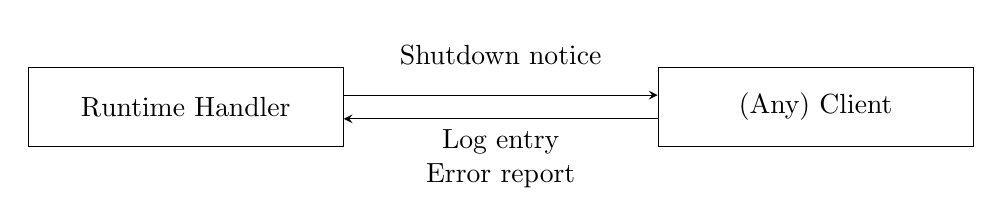
\begin{tikzpicture}[->, >=stealth, rectangle, every node/.style={minimum height=1cm, minimum width=4cm}, node distance=8cm, auto]
			
				\node [draw] (H) {Runtime Handler};
				\node [draw] (C) [right of = H] {(Any) Client};

				\draw [transform canvas={yshift=0.15cm}] (H) edge node[above, align=center]
				{Shutdown notice} (C);
				
				\draw [transform canvas={yshift=-0.15cm}] (C) edge node[below, align=center]
				{Log entry\\Error report} (H);
				
			\end{tikzpicture}
			\caption*{\emph{Possible simple messages between handler and bot- or engine client}}
		\end{figure}
		
		\begin{figure}[H]
			\centering
			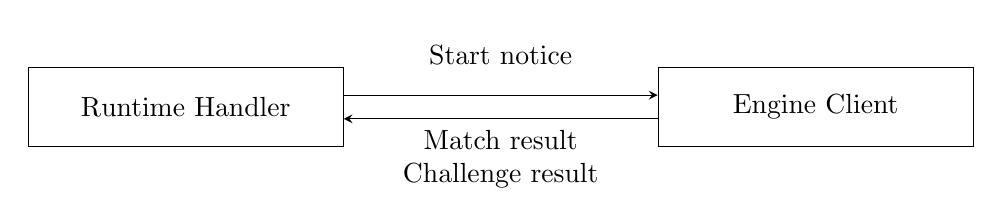
\begin{tikzpicture}[->, >=stealth, rectangle, every node/.style={minimum height=1cm, minimum width=4cm}, node distance=8cm, auto]
			
				\node [draw] (H) {Runtime Handler};
				\node [draw] (EC) [right of = H] {Engine Client};

				\draw [transform canvas={yshift=0.15cm}] (H) edge node[above, align=center]
				{Start notice} (EC);
				
				\draw [transform canvas={yshift=-0.15cm}] (EC) edge node[below, align=center]
				{Match result\\Challenge result} (H);
				
			\end{tikzpicture}
			\caption*{\emph{Possible simple messages between handler and engine client}}
		\end{figure}
		
			\paragraph{Start notice}
			
			This message is only sent once per game to the engine client, as a signal that all actor clients have received all the data (api and actor binaries) that they needed to start working, and a game may be started. Following its reception, the engine client starts the game by invoking the engine object's \code{playGame} method.
		
			\paragraph{Shutdown notice}
			
			This message can be sent at any time during the game, and signals its end --- either due to some error happening or normal game completion --- to the clients, who after receiving it should finish all running tasks, and stop themselves.
		
			\paragraph{Log entry}
			
			Log messages are the only non-control messages, due to them not affecting the flow of the game in any way. They carry their target (the actor or actors whose log will contain the message) and their message itself as their payload. They are sent at any time by one of the actor clients, and are processed independently of the control messages by the runtime handler.
			
			\paragraph{Error report}
			
			Much like log entries, error reports can be sent at any time; however, instead of being actor initiated, they are generated by the client runtime if any irregularity has happened. They can be caused by execptions thrown in the actors' code, unexpected runtime behavior, or attempted access to guarded resources by the actor. As they signal unrecoverable errors, the runtime handler will interrupt the game after receiving them, and choose a result fitting the context the report was created in and the information it carries.
			Based on these pieces of information, the handler will generally mark the game as ended with:
			
			\begin{itemize}
				\item An error caused defeat of the bot of the report's sender (e.g. in case of attempted permission violation or general exception in the bot's code).
				
				\item An error (no winner or loser) if the error occurred not in the actor's, but in the runtime's code
				
				\item Game error if the report was sent from the engine's client due to the former's failure. 
			\end{itemize}
			
			\paragraph{Match result, Challenge result}
			
			Signals from the engine client that imply the engine object's \code{playGame} method successfully finished. They carry the data containing the game's result in accordance with the game model's description. If no error has happened, they act as the signal for the end of the game, and as such may be viewed to form a non-simple message pair with start notice.
			
		\subsection*{Actor binary transfer}
		
		Actor binary messages serve as both parts of a request--response pair. When making a request, a client asks the handler for a type of binary resource required to do its job --- the game's api, engine, or the managed bot. The handler in return sends back the requested binary, while also keeping track of all such requests. If all needed binaries have been sent to all clients, the handler will initialize the start of the game using a start notice message. 
		
		\begin{figure}[H]
			\centering
			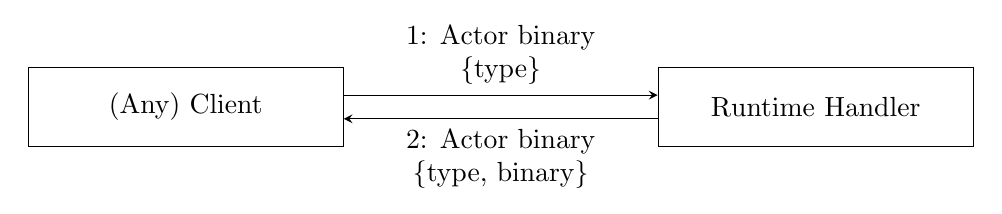
\begin{tikzpicture}[->, >=stealth, rectangle, every node/.style={minimum height=1cm, minimum width=4cm}, node distance=8cm, auto]
			
				\node [draw] (C) {(Any) Client};
				\node [draw] (H) [right of = C] {Runtime Handler};

				\draw [transform canvas={yshift=0.15cm}] (C) edge node[above, align=center]
				{1: Actor binary\\\{type\}} (H);
				
				\draw [transform canvas={yshift=-0.15cm}] (H) edge node[below, align=center]
				{2: Actor binary\\ \{type, binary\} } (C);
				
			\end{tikzpicture}
			\caption*{\emph{Actor binary request--response}}
		\end{figure}
		
		\subsection*{Remote invocation}

		Remote invocation is the most complex communication operation as it involves routing by the handler, and multiple possible valid return types.
		
		As the engine runtime's proxy captures a method call attempt by the engine object, the client sends a proxy call message containing the target bot, requested method identifier, and optional method parameters. This message is forwarded by the handler to the target client, who executes its bot's appropriate method. If this method produces a valid result under the configurable time limit, that value is returned wrapped into a call result message, all the way to the engine. If some error happens during the evaluation, (as usual) an error report is returned to the handler.
		
		However, a special case is also possible, if the bot's method does not finish in time. If this happens, instead of an error report, a bot timeout message is sent back to the engine. This bot timeout acts as a 'recoverable error' --- an event when the engine can choose to ignore the bot's shortcoming. If the engine was created without support for these occurrences, the default error processing takes place.
		
		\begin{adjustwidth}{-0.8cm}{}
		\begin{minipage}[t]{.45\textwidth}
			\begin{figure}[H]
				\centering
				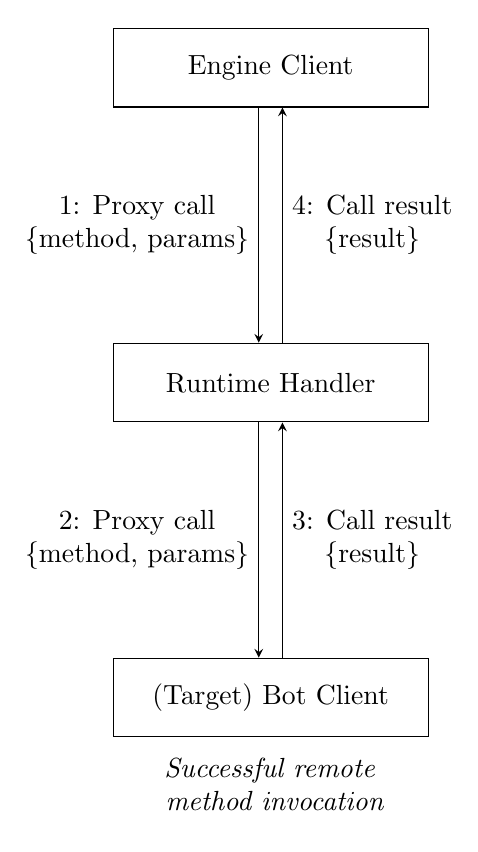
\begin{tikzpicture}[->, >=stealth, rectangle, every node/.style={minimum height=1cm, minimum width=4cm}, node distance=8cm, auto]
			
					\node [draw] (E) {Engine Client};
					\node [draw] (H) [below of = E, node distance=4cm] {Runtime Handler};
					\node [draw] (B) [below of = H, node distance=4cm] {(Target) Bot Client};

					\draw [transform canvas={xshift=-0.15cm}] (E) edge
					node[left, align=center, minimum width=0cm]
					{1: Proxy call \\ \{method, params\}} (H);
				
					\draw [transform canvas={xshift=0.15cm}] (H) edge
					node[right, align=center, minimum width=0cm]
					{4: Call result \\ \{result\}} (E);
				
					\draw [transform canvas={xshift=-0.15cm}] (H) edge
					node[left, align=center, minimum width=0cm]
					{2: Proxy call \\ \{method, params\}} (B);
				
					\draw [transform canvas={xshift=0.15cm}] (B) edge
					node[right, align=center, minimum width=0cm]
					{3: Call result \\ \{result\}} (H);
				
					\node [node distance=1.1cm, align=center] () [below of = B]
					{\emph{Successful remote} \\ \emph{ method invocation}};
				
				\end{tikzpicture}
			\end{figure}
		\end{minipage}\hfill
		\begin{minipage}[t]{.45\textwidth}
			\begin{figure}[H]
				\centering
				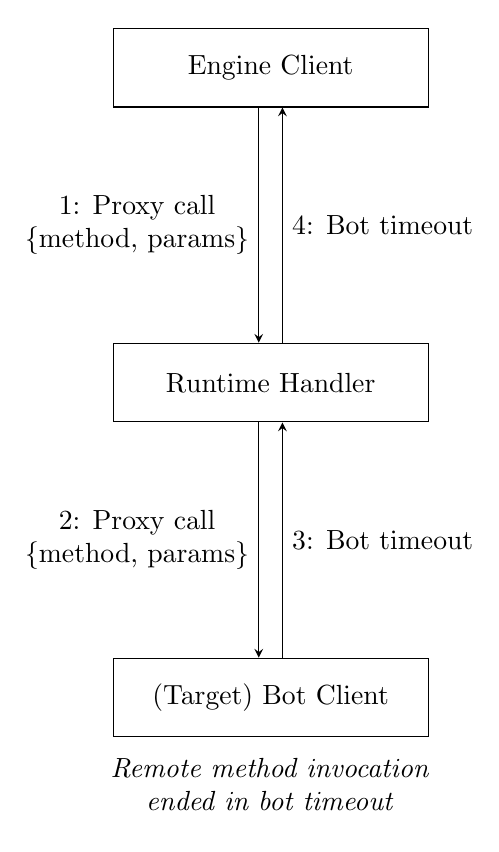
\begin{tikzpicture}[->, >=stealth, rectangle, every node/.style={minimum height=1cm, minimum width=4cm}, node distance=8cm, auto]
			
					\node [draw] (E) {Engine Client};
					\node [draw] (H) [below of = E, node distance=4cm] {Runtime Handler};
					\node [draw] (B) [below of = H, node distance=4cm] {(Target) Bot Client};

					\draw [transform canvas={xshift=-0.15cm}] (E) edge
					node[left, align=center, minimum width=0cm]
					{1: Proxy call \\ \{method, params\}} (H);
			
					\draw [transform canvas={xshift=0.15cm}] (H) edge
					node[right, align=center, minimum width=0cm]
					{4: Bot timeout} (E);
			
					\draw [transform canvas={xshift=-0.15cm}] (H) edge
					node[left, align=center, minimum width=0cm]
					{2: Proxy call \\ \{method, params\}} (B);
			
					\draw [transform canvas={xshift=0.15cm}] (B) edge
					node[right, align=center, minimum width=0cm]
					{3: Bot timeout} (H);
				
					\node [node distance=1.1cm, align=center] () [below of = B]
					{\emph{Remote method invocation} \\ \emph{ended in bot timeout}};
				
			\end{tikzpicture}
			\end{figure}
		\end{minipage}
		\end{adjustwidth}

%\end{document}







%\documentclass[11pt,a4paper,oneside]{report}

%\usepackage[dvipsnames]{xcolor}
%\usepackage{amsmath}
%\usepackage{multirow}
%\usepackage{caption}
%\usepackage{tabularx}
%\usepackage{tikz}
%\usepackage{setspace}

%\usepackage{listings}

%\definecolor{mtypecolor}{HTML}{491b68}
%\definecolor{mtypeparamcolor}{HTML}{1e5b0e}
%\definecolor{mdatasizecolor}{HTML}{aa5908}
%\definecolor{mdatacolor}{HTML}{c40f0f}

%\newcommand{\code}{\texttt}

%\newcommand*{\xdash}[1][5em]{\rule[0.5ex]{#1}{0.55pt}}
%\def\emptycell{\multicolumn{1}{c|}{\xdash}}

%\usetikzlibrary{arrows,positioning, shapes.symbols,shapes.callouts,patterns,calc, automata}

%\lstdefinelanguage{Kotlin}{
%  comment=[l]{//},
%  commentstyle={\color{gray}\ttfamily},
%  emph={delegate, filter, first, firstOrNull, forEach, lazy, map, mapNotNull, println, return@},
%  emphstyle={\color{OrangeRed}},
%  identifierstyle=\color{black},
%  keywords={abstract, actual, as, as?, break, by, class, companion, continue, data, do, dynamic, else, enum, expect, false, final, for, fun, get, if, import, in, interface, internal, is, null, object, override, package, private, public, return, set, super, suspend, this, throw, true, try, typealias, val, var, vararg, when, where, while},
%  keywordstyle={\color{NavyBlue}\bfseries},
%  morecomment=[s]{/*}{*/},
%  morestring=[b]",
%  morestring=[s]{"""*}{*"""},
%  ndkeywords={@Deprecated, @JvmField, @JvmName, @JvmOverloads, @JvmStatic, @JvmSynthetic, Array, Byte, Double, Float, Int, Integer, Iterable, Long, Runnable, Short, String},
%  ndkeywordstyle={\color{BurntOrange}\bfseries},
%  sensitive=true,
%  stringstyle={\color{ForestGreen}\ttfamily},
%}

%\lstset{basicstyle=\footnotesize\ttfamily,breaklines=true}
%\lstset{framextopmargin=5pt, framexleftmargin=5pt, framexrightmargin=5pt, framexbottommargin=5pt, frame=bottomline}
%\lstset{language=Kotlin, frame=single, gobble=4, tabsize=4, showstringspaces=false}

%\begin{document}
%\onehalfspacing
%----------------------------------------------------------------------------
\chapter{Runtime Implementation}\label{sect:RuntimeImpl}
%----------------------------------------------------------------------------

	\section{Messaging}
		\subsection{Format}
		
		All messages start with a fixed prefix (\code{MESSAGE}), end with a line break, and their different parts are separated by hyphens. Messages consist of two logical parts: the header and the payload. The former specifies the type of the message, and provides other information like the type parameters which may be needed to process this kind of message; while the latter carries additional information in the form of a blob and its size in bytes.
		
		\begin{figure}[h]
			\[
				\code{MESSAGE-}%
				\overbrace{\text{\code{%
					\color{mtypecolor}\{Message type\}\color{black}-%
					(\color{mtypeparamcolor}\{Type parameter\}\color{black}-)*%	
				}}}^{\text{Header}}%
				\overbrace{\text{\code{%
					\color{mdatasizecolor}\{Data size\}\color{black}-%
					\color{mdatacolor}\{Data\}?%
				}}}^{\text{Payload}}%\text{\code{\textbackslash n}}%
			\]
			\caption*{\emph{Structure of the messages}}
		\end{figure}
		
		\paragraph{Type parameters and payload}
		
		The difference between the type parameters and the payload data is that type parameters can be understood and processed without 'unsafe' operations such as java deserialization. Their arity and types are determined by the message type, and their values may consist of primitives, strings, or values of enumerations. This --- combined with a size limit on them --- allows the runtime handler to always safely parse, process and, optionally, route the messages without requiring it to understand the potentially unsafe data of the payload.
		
		The data payload on the other hand deals with binary data produced by one of the actors, and as such should only be parsed by the actor clients taht are already equipped with the proper protective capabilities.
		The payloads size --- in bytes --- is also included in the message for safe message handling.
		
		Both the type parameters and the payload are converted to base 64 strings, as to make message formatting and parsing easier --- due to no necessary separator escaping.
		
		\begin{table}[h]
			\centering
			\setlength{\tabcolsep}{8pt}
			\renewcommand{\arraystretch}{1.5}
			\begin{tabularx}{\linewidth}{
				|>{\hsize=0.8\hsize}X|% 
				>{\hsize=0.8\hsize}X|%
				>{\hsize=1.4\hsize}X|%
			  }
				\hline
				 \multicolumn{1}{|c|}{\textbf{Message type}} &%
				 \multicolumn{1}{c|}{\textbf{Parameters}} &%
				 \multicolumn{1}{c|}{\textbf{Payload}} \\ \hline
				
				Start notice & \emptycell & \emptycell \\ \hline
				Shutdown notice & \emptycell & \emptycell \\ \hline
				
				\multirow{2}{*}{Log entry} & Target actor & \multicolumn{1}{c|}{\multirow{2}{*}{\xdash}} \\
					& Log message & \\ \hline
				
				Error report & Error message & \emptycell \\ \hline
				
				\multirow{2}{*}{Challenge result} & Points & \multicolumn{1}{c|}{\multirow{2}{*}{\xdash}} \\
					& Max points & \\ \hline
				
				Match result & Three way result & \emptycell \\ \hline
				Actor binary & Type & Binary (nothing on requests) \\ \hline
				
				\multirow{2}{*}{Proxy call} & \multirow{2}{*}{Target bot} & Target method \\
					& & Call parameters \\ \hline
				
				Call result & Called method & Result data \\ \hline
				
				Bot timeout & \emptycell & \emptycell \\ \hline
			\end{tabularx}
			\caption*{\emph{Type parameters and payloads of message types}}
		\end{table}

		\subsection{Conversion and serialization}
		
			\paragraph{Conversion and deconversion}
		
			Conversion is the process during which domain representation of a message in the form of a \code{Message} object is converted into an intermediate state as it gets ready to be sent. Its result is a \code{MessageDTO}, an object which holds the same header the original message did, but has its payload --- if any were present --- transformed into a processable, base 64 encoded string representation. Deconversion is its inverse operation. It is a distinct process from the general serialization of messages, as to ensure independence between the algorithms used in the two processes.
			
			This loose coupling is beneficial, as conversion is an unsafe routine that only actor clients should conduct. Message (de)conversion is required when dealing with remote proxy calls, and this breakup of concerns allows the runtime handler to parse and route a call request or call result message without attempting to decode its payload, which contains JVM objects as transformed by standard java serialization. As object (de)serialization is dangerous --- due to the construction of arbitrary large serialization 'bombs' ---, it is best to pass these messages to the actor clients who are equipped with proper security measures to safely minister it.

			\paragraph{Serialization and Deserialization}
			
			Serialization takes payload-less messages or converted messages, and transforms them to the aforementioned general message format. This includes encoding the message header, and concatenating it to the prefix and optional (already converted) payload. This encoding of the header --- and its pair decoding in deserialization --- can be done safely and strictly, as the content of the header specified by the message type, and its parameters are simple values that can be easily converted to strings.
			
			As all parties require (de)serialization to communicate, the components providing these services are shared across all of them.

		\subsection{Communication}
		
		All messaging is done over point-to-point, full-duplex TCP channels between the actor clients and the runtime handler. These connections are initialized by the clients, who as a command argument receive the host --- usually localhost --- and the port they should connect to. These ports are free ports chosen randomly by the handler, and reserved before the start of the clients.
		
		Once these channels have been established, communication should begin as described by the communication model --- starting with the clients requesting the game specific actor binaries.
		
		If a game if finished --- in a normal way or because of errors ---, or a communication channel should fail (e.g. due to unexpected crash of an actor), the runtime notifies all (still reachable) clients with shutdown notices. After sending and receiving these, all participants are to assume the game has ended, the clients stop themselves, and the handler reports the result of the challenge or match.

		Just like serialization, low level communication is helped by components shared across all members of the runtime model.

	\section{Runtime handler}

	A runtime handler is made up of a couple of active components and passive data structures. Active components are primarily based on their own thread, and communicate with each other through either direct calls, or the passive structures.
	There are two kinds of these active components, a --- per runtime handler --- singleton control handler, and actor handlers for each actor client runtime. Passive components come in the form of a control queue and log stores for each actor.
		
		\begin{figure}[h]
			\centering
			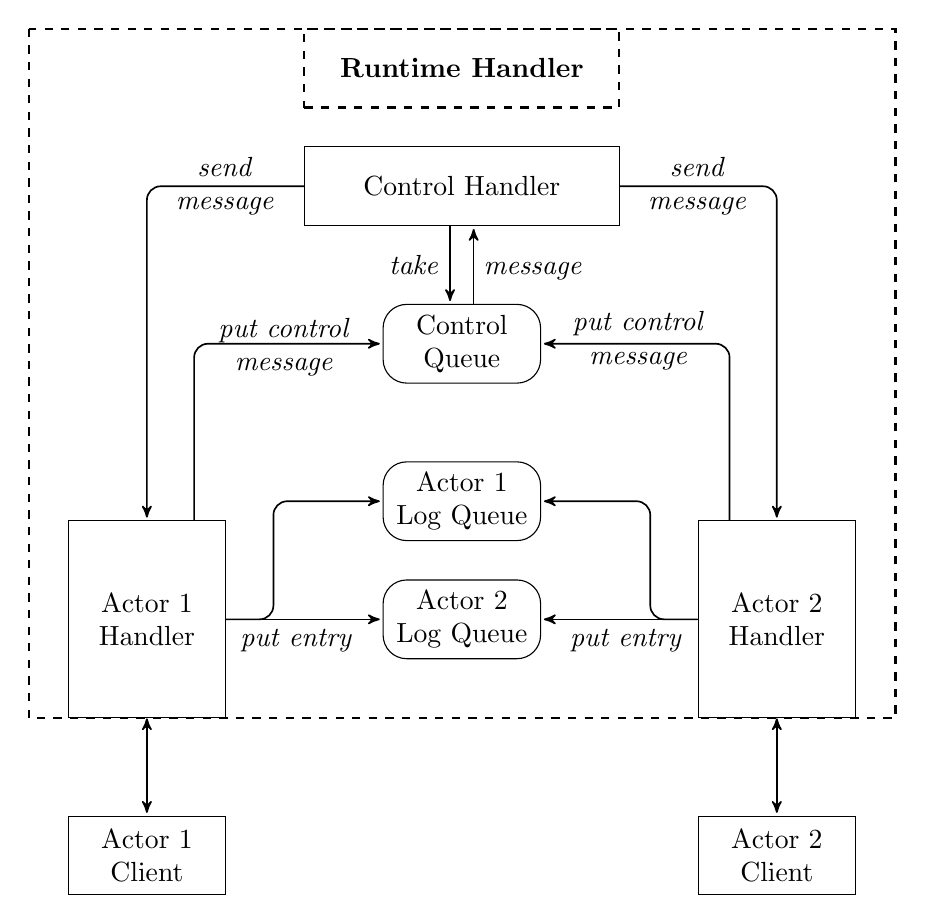
\begin{tikzpicture}[->, >=stealth, rectangle, every node/.style={minimum height=1cm, minimum width=4cm}, node distance=2cm, auto, post/.style={->,shorten >=1pt,>=stealth',semithick}]
			
				\node [draw] (CH) {Control Handler};
				\node [draw] (CQ) [below of = CH, node distance=2cm, minimum width=2cm, align=center, rounded corners=.3cm]
					{Control\\Queue};
				
				\node [draw] (A1LQ)
					[below of = CQ, node distance=2cm, align=center, minimum width=2cm, rounded corners=.3cm]
					{Actor 1 \\ Log Queue};
				
				\node [draw] (A2LQ)
					[below of = A1LQ, node distance=1.5cm, align=center, minimum width=2cm, rounded corners=.3cm]
					{Actor 2 \\ Log Queue};
				
				\node [draw] (A1H)
					[left of=A2LQ, node distance=4cm, align=center, minimum width=2cm, minimum height=2.5cm]
					{Actor 1 \\ Handler};
				
				\node [draw] (A2H)
					[right of=A2LQ, node distance=4cm, align=center, minimum width=2cm, minimum height=2.5cm]
					{Actor 2 \\ Handler};
				
				\node [draw] (A1C)
					[below of=A1H, node distance=3cm, align=center, minimum width=2cm]
					{Actor 1 \\ Client};
				
				\node [draw] (A2C)
					[below of=A2H, node distance=3cm, align=center, minimum width=2cm]
					{Actor 2 \\ Client};
				
				\draw[post] (CH) edge [transform canvas={xshift=-0.15cm}]
					node [left, minimum width=0cm] {\emph{take}} (CQ);
				\draw[post] (CQ) edge [transform canvas={xshift=0.15cm}]
					node [right, transform canvas={yshift=-0.08cm}] [minimum width=0cm] {\emph{message}} (CH);
				
				\draw[post,rounded corners=5pt] (CH) node [align=center, transform canvas={xshift=-3cm}] 
					{\emph{send}\\ \emph{message}} -| (A1H);
				\draw[post,rounded corners=5pt] (CH) node [align=center, transform canvas={xshift=3cm}] 
					{\emph{send}\\ \emph{message}} -| (A2H);
				
				\draw[post,rounded corners=5pt] (A1H.north) ++(.6,0) |-
					node [transform canvas={xshift=1.15cm, yshift=-0.55cm}, align=center]
					{\emph{put control}\\ \emph{message}} (CQ);
				\draw[post,rounded corners=5pt] (A2H.north) ++(-.6,0) |- 
					node [transform canvas={xshift=-1.15cm, yshift=0.55cm}, align=center]
					{\emph{put control}\\ \emph{message}} (CQ);
				
				\draw[post,rounded corners=5pt] (A1H.east) -- ++(.6,0) |- (A1LQ);
				\draw[post] (A1H.east) node [minimum height=0cm, below, transform canvas={xshift=0.9cm}]
					{\emph{put entry}} |- (A2LQ);
				
				\draw[post,rounded corners=5pt] (A2H.west) -- ++(-.6,0) |- (A1LQ);
				\draw[post] (A2H.west) node [minimum height=0cm, below, transform canvas={xshift=-0.9cm}]
					{\emph{put entry}} |- (A2LQ);
				
				\draw[post, <->] (A1H) edge (A1C);
				\draw[post, <->] (A2H) edge (A2C);
				
			    \draw[thick, dashed] (-5.5cm,2cm) rectangle ($(A2H.south east) + (0.5,0)$);
				\node[draw, dashed, thick] (T) [above of=CH, node distance=1.5cm] {\textbf{Runtime Handler}};
				
			\end{tikzpicture}
			\caption*{\emph{Runtime handler simplified component model} \\ \emph{Challenge -- two actors}}
		\end{figure}
		
		\subsection{Control handler}
		
		The control handler is the heart of the runtime handler, as its name implies, it directs the flow of the game, and manages the actor handlers. At its core it is a finite-state machine that processes control messages, and optionally instructs the actor handlers to send messages based on the actions.
		
		It is important to note that the control messages it consumes are slightly different from the general messages sent between the members of the runtime model, as they have been preprocessed by the actor handlers. The two main changes are that log messages have been removed (they are processed by the actor handlers), and each message contains its source actor. The control handler acquires these messages from the control queue, which acts as a thread-safe buffer between the components. The possible control states are:
		
		\begin{itemize}
			\item \textbf{Connection await} The initial state, it signals that not all actor clients are ready to start, as not all have connected or received all the binaries they need.
			
			\item \textbf{Wait for Engine} The engine is working.

			\item \textbf{Wait for Bot} The engine had requested a proxy call, whose result has not been returned from the target bot's actor yet.
			
			\item \textbf{Finished} The game had finished normally. \emph{End}
			
			\item \textbf{Crash} The game finished abnormally due to some error. \emph{End}
		\end{itemize}

		\begin{figure}[h]
			\centering
			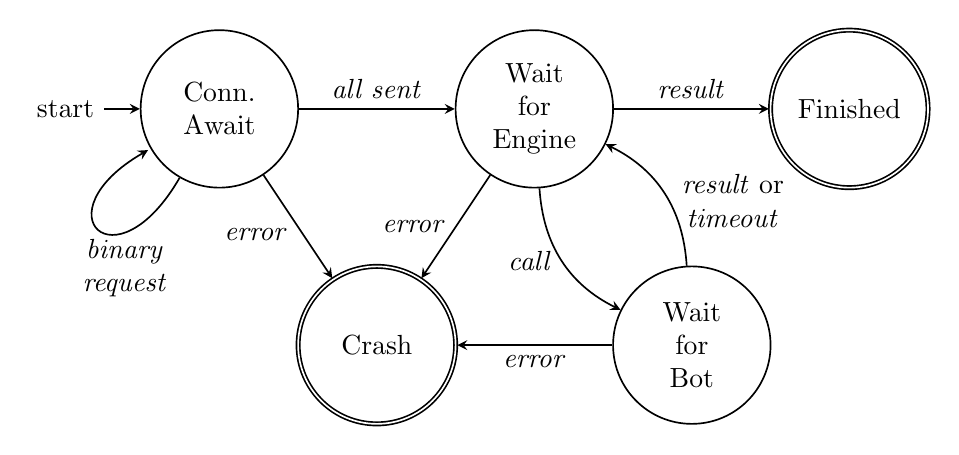
\begin{tikzpicture}[->, >=stealth, node distance=4cm, auto, semithick, state/.style={circle, draw, minimum size=2cm}]
				\pgfmathtruncatemacro{\last}{4}		
		
				\node[state, initial, align=center] (ConnAwait)
					{Conn. \\ Await};
				\draw (ConnAwait) edge [in=210,out=240,loop] node [align=center, xshift=1cm]
					{\emph{binary} \\ \emph{request}} (ConnAwait);
		
				\node[state, right of=ConnAwait, align=center] (WaitEngine) {Wait \\ for \\ Engine};
		
				\node[state, right of=WaitEngine, align=center, accepting] (Done)
					{Finished};
		
				\node[state, below of=ConnAwait, node distance=3cm, align=center, accepting] (Crash)
					at ($(ConnAwait)!0.5!(WaitEngine)$) {Crash};
		
				\node[state, below of=WaitEngine, node distance=3cm, align=center] (WaitBot)
					at ($(WaitEngine)!0.5!(Done)$) {Wait \\ for \\ Bot};
		
				\draw (ConnAwait) edge node {\emph{all sent}} (WaitEngine);
				\draw (WaitEngine) edge node {\emph{result}} (Done);
		
				\draw (ConnAwait) edge node [left, yshift=-0.1cm] {\emph{error}} (Crash);
				\draw (WaitEngine) edge node [left] {\emph{error}} (Crash);
				\draw (WaitBot) edge node [below] {\emph{error}} (Crash);
		
				\draw (WaitEngine) edge [bend right] node [left] {\emph{call}} (WaitBot);
				\draw (WaitBot) edge [bend right] node [right, align=center, xshift=0.1cm, yshift=-0.1cm]
					{\emph{result} or \\ \emph{timeout}} (WaitEngine);
		
			\end{tikzpicture}
			\caption*{\emph{Control state machine}}
		\end{figure}

		To simplify game flow management, the control handler is an extended state machine, which allows states to store variables as internal state. This data allows for selective transitions to happen, and help store results in the final (accepting) states. Each state may have its own set of parameters as follows: 

		\begin{table}[h]
			\centering
			\setlength{\tabcolsep}{8pt}
			\renewcommand{\arraystretch}{1.5}
			\begin{tabularx}{0.8\linewidth}{
				|>{\hsize=0.7\hsize}X|% 
				>{\hsize1.3\hsize}X|%
			  }
				\hline
				 \multicolumn{1}{|c|}{\textbf{Control state}} &%
				 \multicolumn{1}{c|}{\textbf{Parameters}} \\ \hline
				
				Connection await & sent binaries by receiver client \\ \hline
				Wait for Engine & \emptycell \\ \hline
				Wait for Bot & target bot, called method \\ \hline
				Finished & challenge/match result \\ \hline
				Crash & optional result, error description \\ \hline
			\end{tabularx}
			\caption*{\emph{Parameters of control states}}
		\end{table}

			\paragraph{Game flow}
			
			The controller starts off in the \code{Connection await} state, and remains there until all actors have received their required binaries. It keeps track of the sent libraries, and after the last of these has been issued, a 'Start notice' message is sent to the engine client, the state is changed to \code{Wait for Engine}, and the game starts.
			
			During the game, as the engine makes calls for which the bots respond, the state is bouncing between \code{Wait for Engine} and \code{Wait for Bot}. As a security measure, the target bot and called method are also stored, so that it can be verified that the right bot answered a call. As per the game model, 'Bot timeout' messages are also possible in the place of 'Call results'.
			
			After the game had come to a conclusion, and the engine had sent the proper result message, the state reaches \code{Finished}, where it stays while keeping the game result.
			
			Of course while in any active state, an error might also happen, in which case the controller changes to the \code{Crash} state. Although in this case a game result have not been reported by the engine, the controller might set a valid result anyway, based on the context in which the error occurred. If for example the game crashed due to a runtime exception while executing a code of a bot, the result of the challenge or match will be set to error from that bot --- a result that is processed similarly to the opponent winning in the case of a match, or a 0 point run in the case of a challenge.

		\subsection{Actor handler}

		In contrast to the control handler, separate actor handlers are created for each actor. These composite components are responsible for communicating with the runtime clients, processing incoming messages, storing log entries, and forwarding control messages to the control handler in a digestible format.
		
		Low level communication with the clients is done using a channel, an object which provides a safe, message-aware wrapper for the underlining network sockets. On top of this sits a message handler, which now provides operations based on the type of the clients (engine or bot). This handler is accessed by two components, the already mentioned control handler and the message router receiver. Both of these objects run on their own threads while using the message handler, but due to them only using the sending or receiving capabilities respectively (and the fact that the underlying architecture is full-duplex capable), these actions can happen independently. The message router receiver's thread can be considered the actor handler's main thread, as it performs most of the tasks of the handler. It blockingly waits for incoming messages, then routes them according their purpose. 

		Control messages get transcribed into the format the control handler can understand, and put onto the control queue from where they will be taken by the control handler. Log messages on the other hand are passed to a log router, an object which puts them into their target's log queue. As game engines have the power to simultaneously send info entries to multiple actors, this might mean more than one overall targets.
		
		Actor handlers are designed to be as reusable as possible when dealing with different types of actors. This means that only the message handler and the log router differ based on actor kind --- as they either must show different sending methods to the outside, or must work fundamentally differently while routing messages. Also their characteristics are hidden from the other components (except for the control handler) via abstraction achieved by the inheritance of a base type. 

		\begin{figure}[h]
			\centering
			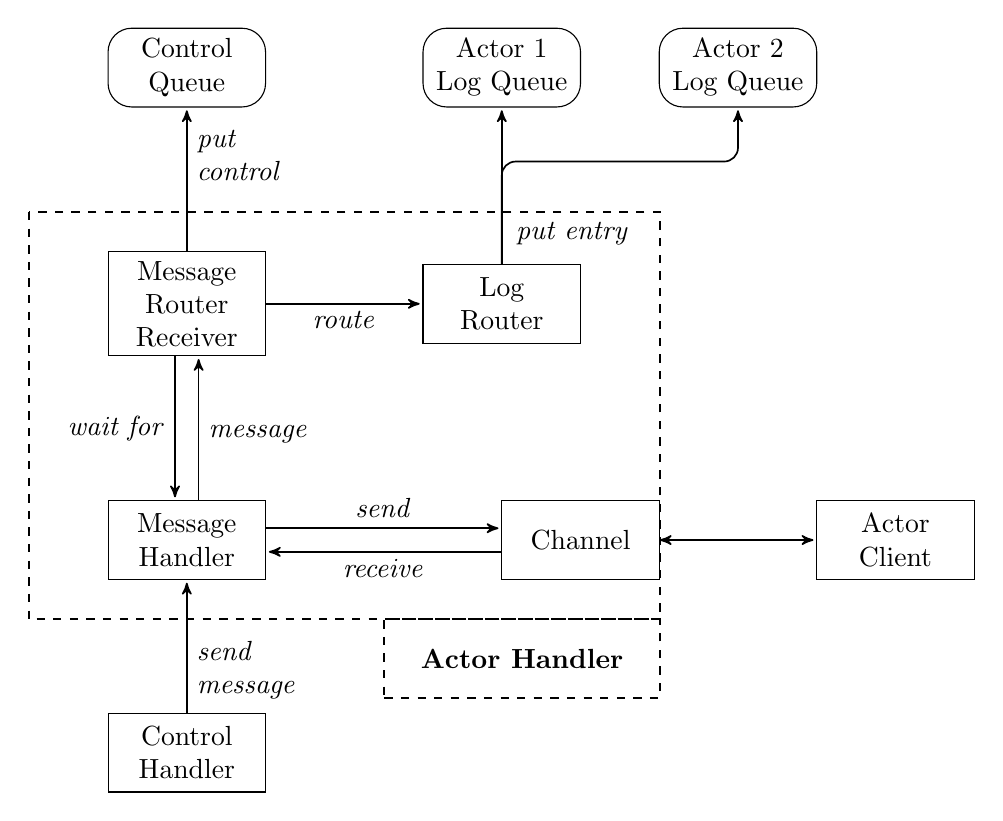
\begin{tikzpicture}[->, >=stealth, rectangle, every node/.style={minimum height=1cm, minimum width=4cm}, node distance=2cm, auto, post/.style={->,shorten >=1pt,>=stealth',semithick}]
			
				\node [draw] (CQ) [minimum width=2cm, align=center, rounded corners=.3cm]
					{Control\\Queue};
				
				\node [draw] (A1LQ)
					[node distance=4cm, right of=CQ, minimum width=2cm, align=center, rounded corners=.3cm]
					{Actor 1\\Log Queue};
				
				\node [draw] (A2LQ)
					[node distance=3cm, right of=A1LQ, minimum width=2cm, align=center, rounded corners=.3cm]
					{Actor 2\\Log Queue};
				
				\node [draw] (MRR)
					[node distance=3cm, below of=CQ, minimum width=2cm, align=center]
					{Message\\Router\\Receiver};
				
				\node [draw] (LR)
					[node distance=4cm, right of=MRR, minimum width=2cm, align=center]
					{Log\\Router};

				\node [draw] (MH)
					[node distance=3cm, below of=MRR, minimum width=2cm, align=center]
					{Message\\Handler};
				
				\node [draw] (C)
					[node distance=5cm, right of=MH, minimum width=2cm, align=center]
					{Channel};
				
				\node [draw] (AC)
					[node distance=4cm, right of=C, minimum width=2cm, align=center]
					{Actor\\Client};
				
				\node [draw] (CH)
					[node distance=2.7cm, below of=MH, minimum width=2cm, align=center]
					{Control\\Handler};
				
				\draw[post] (MRR) edge [right] node [minimum width=0cm, align=left, yshift=0.3cm]
					{\emph{put}\\ \emph{control}} (CQ);
				
				\draw[post] (MRR) edge [below] node [minimum width=0cm, align=center, yshift=0.3cm]
					{\emph{route}} (LR);
				
				\draw[post] (LR) edge [below] node
					[minimum width=0cm, align=center, yshift=-0.1cm, xshift=0.9cm]
					{\emph{put entry}} (A1LQ);
					
				\draw[post,rounded corners=5pt] (LR.north) -- ++(0,1.3) -| (A2LQ.south);
				
				\draw[post] (MRR) edge [transform canvas={xshift=-0.15cm}]
					node [left, minimum width=0cm] {\emph{wait for}} (MH);
				\draw[post] (MH) edge [transform canvas={xshift=0.15cm}]
					node [right, transform canvas={yshift=-0.08cm}, minimum width=0cm] {\emph{message}} (MRR);
				
				\draw[post] (MH) edge [transform canvas={yshift=0.15cm}]
					node [above, minimum width=0cm, yshift=-0.25cm] {\emph{send}} (C);
				\draw[post] (C) edge [transform canvas={yshift=-0.15cm}]
					node [below, transform canvas={yshift=0.3cm}, minimum width=0cm] {\emph{receive}} (MH);
				
				\draw[post] (CH) edge [right] node [minimum width=0cm, yshift=-0.3cm, align=left]
					{\emph{send}\\ \emph{message}} (MH);
				
				\draw[post, <->] (C) edge (AC);
				
				\draw[thick, dashed] ($(MRR.north west) + (-1,0.5)$) rectangle ($(C.south east) + (0,-0.5)$);
				\node[draw, dashed, thick] (T) [below = of C.east, anchor=east, minimum width=3.5cm, yshift=0.495cm, xshift=0.015cm]
					{\textbf{Actor Handler}};
				
			\end{tikzpicture}
			\caption*{\emph{Actor handler model} \\ \emph{Challenge -- two actors}}
		\end{figure}		
		
	\section{Actor runtime}

	The structure of actor runtimes is fairly simple, and is largely identical between engine- and bot clients. Their core component is the 'client', which provides the logic necessary to manage the actor assigned to them, and therefore of course contains actor role (engine or bot) specific code. The rest of the components involved in the communication process are equivalent in each case. The client is based on three active objects all running on separate threads --- a message receiver, a message sender, and the aforementioned client. These elements are communicating with each other --- in a one-way manner --- over blocking queues.
	
	The receiver waits for messages over the communication channel, processes them and places them on the 'In queue', from where the client can get them. It may also initiate the exit of the client if a shutdown notice is received. Likewise, the sender sends messages placed onto the 'Out queue' by the client.
		
	\begin{figure}[h]
		\centering
		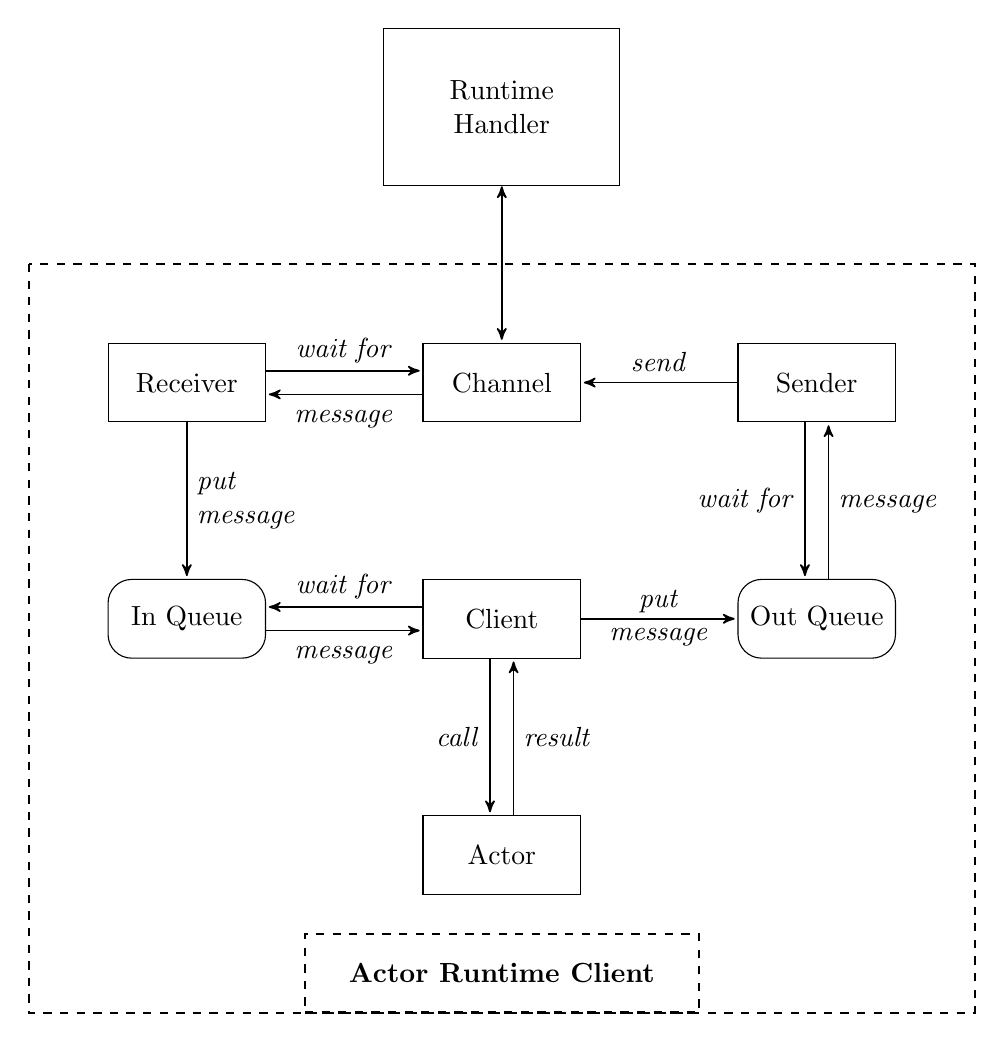
\begin{tikzpicture}[->, >=stealth, rectangle,
							every node/.style={minimum height=1cm, minimum width=2cm, align=center},
							node distance=3cm, auto,
							post/.style={->,shorten >=1pt,>=stealth',semithick},
							passive/.style={rounded corners=.3cm}]
		
			\node [draw] (RH) [minimum width=3cm, minimum height=2cm] {Runtime\\Handler};
			
			\node [draw] (C) [below of=RH, node distance=3.5cm] {Channel};
			
			\node [draw] (R) [left of=C, node distance=4cm] {Receiver};
			
			\node [draw] (S) [right of=C, node distance=4cm] {Sender};
				
			\node [draw, passive] (In) [below of=R] {In Queue};
				
			\node [draw, passive] (Out) [below of=S] {Out Queue};
				
			\node [draw] (CL) [below of=C] {Client};
				
			\node [draw] (A) [below of=CL] {Actor};
				
			\draw[post] (RH) edge [<->] (C);
			 
			\draw[post] (R) edge [transform canvas={yshift=0.15cm}]
				node [above, yshift=-0.25cm] {\emph{wait for}} (C);
			\draw[post] (C) edge [transform canvas={yshift=-0.15cm}]
				node [below, yshift=0.2cm] {\emph{message}} (R);
			
			\draw[post] (S) edge node [above, yshift=-0.25cm] {\emph{send}} (C);
			
			\draw[post] (R) edge node [align=left, minimum width=0cm] {\emph{put} \\ \emph{message}} (In);
			
			\draw[post] (S) edge [transform canvas={xshift=0-.15cm}]
				node [left, align=right, minimum width=0cm] {\emph{wait for}} (Out);
			\draw[post] (Out) edge [transform canvas={xshift=0.15cm}]
				node [right, align=left, minimum width=0cm, yshift=-0.05cm] {\emph{message}} (S);
							
			\draw[post] (CL) edge [transform canvas={yshift=0.15cm}]
				node [above, yshift=-0.25cm] {\emph{wait for}} (In);
			\draw[post] (In) edge [transform canvas={yshift=-0.15cm}]
				node [below, yshift=0.2cm] {\emph{message}} (CL);
				
			\draw[post] (CL) edge node [above, yshift=-0.5cm] {\emph{put}\\ \emph{message}} (Out);
					
			\draw[post] (CL) edge [transform canvas={xshift=0-.15cm}]
				node [align=right, left, minimum width=0cm] {\emph{call}} (A);
			\draw[post] (A) edge [transform canvas={xshift=0.15cm}]
				node [align=left, right, minimum width=0cm] {\emph{result}} (CL);
							
			\draw[thick, dashed] ($(R.north west) + (-1,1)$) rectangle ($(A.south east) + (5,-1.5)$);
			\node[draw, dashed, thick] (T)
				[below of = A, node distance=1.5cm, minimum width=5cm]
				{\textbf{Actor Runtime Client}};
								
		\end{tikzpicture}
		\caption*{\emph{Actor runtime client model}}
	\end{figure}
	
		\subsection{Base client}

			As the client's workflow is dependent on the type of the actor it manages, it is realized as two different classes --- the \code{EngineClient} and the \code{BotClient} ---, but many common functions are outsourced from these to shared dependencies.

			\subsubsection*{Class loading and security}
		
			The most important job of all actor clients is the provision of a safe runtime environment where the actor's and the game api's inherently untrusted code may be executed. This is supported by the standard solutions provided by the java virtual machine. The heart of guarding valuable resources (such as files or \mbox{I/O} capabilities), is the strict separation of safe- and unsafe code with their respective permissions assigned.
			
			Safe code is constituted by all the sources of the runtime client and its dependencies, such as java libraries used --- effectively the whole codebase of the runtime. This partition is granted all possible permissions using a policy file, which is --- with the enforcing security manager --- put into effect via program arguments passed to the JVM.

			\begin{center}
				\begin{minipage}{12cm}
					\begin{lstlisting}[language=Java, title={\code{client.policy}}]
	   grant codeBase "file:${trusted.codebase}" {
		   permission java.security.AllPermission "", "";
	   };
					\end{lstlisting}
				\end{minipage}
			\end{center}
		
			This policy grants all permissions to classes whose source URI matches the file path also set as a vm argument through \code{-Dtrusted.codebase}. This property is in turn set by the starter script to the executable jar's path that not only contains the actor client, but also all of its necessary dependencies as well.
			
			As a security manager is installed, other code sources have no granted permissions by default, therefore all other (unsafe) code parts need only not to be marked as being from the same source.
			
			The loading of the user-defined code blocks is implemented by a custom class loader (\code{BinaryClassLoader}), which works on in-memory byte array representations of java archives (JARs). These libraries are sent over to the actor client in actor binary messages, then the client passes them to the classloader for processing. The loader iterates through the compiled referencial type entries of the archive (\code{.class} files), and defines them using the standard native class loader methods. The binary class loader also sets these classes protection domain, which --- due to different source definitions --- provide no granted permissions to them.
			
			Although this way no permissions are granted to the user defined programs, they would still be able to engage in unwanted behavior, namely multi-thread operations. The game model specifies strict 'ask--respond' style communication between the engine and the bots for clear gameplay and enforceable timeout limiting. This means that when --- as a result of a proxy invocation --- a method of a bot is called, it must finish all operations when that method returns. As threads cannot be safely killed once started, this effectively forbids custom thread creation, even in non-straightforward ways, such as the use of an executor framework. Fortunately, while 'no granted permissions' still allow thread creation, there is a safe way of disabling thread formation for unsafe code. At the initialization of a thread object, the environment does check access permission, but the default behavior is to allow thread creation if the thread is created into the current thread group. The look up of the current group is done by the set up security manager using its \code{getThreadGroup} method. By overriding this method of the default security manager, we can return the root thread group, which will always be different from the caller's thread group, and thus thread creation will fail when attempted from unsafe code.
			
		\subsubsection*{Actor initialization}
		
		Initializing an actor instance to manage starts with finding the game's bot interface. This is done by searching through the user defined types, and finding the appropriate class object. This capability is shared between the different types of runtime clients.
		
			\paragraph{Engine client}
		
			After the bot interface has been found, the engine client creates one or two stub instances for this interface. This is done using the java runtime's built-in dynamic proxy creation capability through the \code{Proxy} class' static \code{newProxyInstance} method. This method takes an invocation handler --- a callback that takes as its parameters the context in which a method of the proxy was called, and meta data about that same method. My implementation of this callback is to create and send --- put into the outgoing message queue to be more precise --- a proxy call message. This message will contain the target bot, a unique identifier of the method (full signature), and the method arguments serialized.
			
			After the stubs have been generated, the engine client searches through the user defined classes, looks for the engine, and creates an instance of it with the previously created proxies as the constructor parameters.
			
			\paragraph{Bot client}
			
			The bot client finds the bot implementation that realizes the bot interface (and has a zero argument constructor), and instantizes it. Then the client uses the bot interface to create a skeleton for the remote invocation. This object holds all the bot interface's methods (represented by their unique identifiers, same as on the engine client's side) mapped to the aforementioned bot instance's corresponding methods. When a proxy call message is received, this skeleton executes a lookup of the method identifier, and calls the matching method of the bot, and sends the result back as a call result message. 
			
%\end{document}








%\documentclass[11pt,a4paper,oneside]{report}

%\usepackage[dvipsnames]{xcolor}
%\usepackage{listings}
%\usepackage{setspace}
%\usepackage{caption}
%\usepackage{tabularx}
%\usepackage{amsmath}
%\usepackage{amssymb}
%\usepackage{mathtools}
%\usepackage{graphics}
%\usepackage{anysize}

%\lstdefinelanguage{Kotlin}{
%  comment=[l]{//},
%  commentstyle={\color{gray}\ttfamily},
%  emph={delegate, filter, first, firstOrNull, forEach, lazy, map, mapNotNull, println, return@},
%  emphstyle={\color{OrangeRed}},
%  identifierstyle=\color{black},
%  keywords={open, operator, abstract, actual, as, as?, break, by, class, companion, continue, data, do, dynamic, else, enum, expect, false, final, for, fun, get, if, import, in, interface, internal, is, null, object, override, package, private, public, return, set, super, suspend, this, throw, true, try, typealias, val, var, vararg, when, where, while},
%  keywordstyle={\color{NavyBlue}\bfseries},
%  morecomment=[s]{/*}{*/},
%  morestring=[b]",
%  morestring=[s]{"""*}{*"""},
%  ndkeywords={@Deprecated, @JvmField, @JvmName, @JvmOverloads, @JvmStatic, @JvmSynthetic, Array, Byte, Double, Float, Int, Integer, Iterable, Long, Runnable, Short, String},
%  ndkeywordstyle={\color{BurntOrange}\bfseries},
%  sensitive=true,
%  stringstyle={\color{ForestGreen}\ttfamily},
%}

%\lstset{basicstyle=\footnotesize\ttfamily,breaklines=true}
%\lstset{framextopmargin=5pt, framexleftmargin=5pt, framexrightmargin=5pt, framexbottommargin=5pt, frame=bottomline}
%\lstset{language=Kotlin, frame=single, gobble=4, tabsize=4, showstringspaces=false}

%\newcommand{\code}{\texttt}

%\newcolumntype{Y}{>{\centering\arraybackslash}X}

%\marginsize{35mm}{25mm}{15mm}{15mm} % anysize package

%\begin{document}
%\onehalfspacing

%----------------------------------------------------------------------------
\chapter{Kreator}\label{sect:Kreator}
%----------------------------------------------------------------------------

Parallel to the development of the main project --- and in coordination with it ---, I have started working on a framework to allow well-integrated dependency injection for kotlin.

Although solutions of varying functionality and quality have existed for years --- such as Kodein~\cite{Kodein} or KOIN~\cite{KOIN} for kotlin, and many others for the JVM in general~\cite{JavaCdi} ---, I have found them not to work in accordance of how I would prefer such a library or framework to behave.

	\section{Introduction}
	
	Dependency injection in object oriented environments is usually manifested in providing objects to other objects, where the latter use some accessible services of the former. This pattern can be immensely useful in reducing coupling and module dependency, which in turn allow for easier unit testing, better project transparency, and more.
	
		\subsection*{Types of injection}
		
		Conventionally, dependency injection is separated into three main types: \emph{constructor-}, \emph{setter-}, and \emph{interface injection}~\cite{DiTypes}. These cover most of the options commonly used in the java world, but --- while using for-java libraries is possible, --- due to more powerful language capabilities, solutions in the kotlin ecosystem use different methods. The most important features of kotlin that endorse different patterns are strong immutability support (\code{val}), simplified 'setter constructor' definition --- both incentivizing an in-constructor initialization of dependencies --- and first class singleton support (\code{object}) and top level functions, which allow for easier programmatic injection. Setter- and interface injection is, of course, still possible (through nullable or \code{lateinit} properties), but result in a reduction of code quality.
		
		\subsection*{Categorization}
	
		DI is compromised of two necessary phases: resource declaration and injection. The former is the process in which dependencies are identified for the framework, while injection is the practice of actually providing the requested dependencies, optionally initializing them in the process.
		
		Most available dependency injection solutions work in what I would categorize into one of two ways: declarative- or imperative injection. Declarative injection uses annotations (or in the past, commonly XML configuration) to identify resources, and injects these at marked injection points, such as setters of annotated properties. This kind of injection relies on managed component handling to detect when an injection should occur. On the other hand, imperative injection frameworks require components to be registered at startup to be injectable, and they can be requested via functions.
	
	\section{Design}
	
		Kreator is based on a mixed system where resource identification is done in a declarative way using annotations, while resource injection is implemented in an imperative manner through global functions (\code{inject*}). This aims to capture the best of both words --- easy to understand definition and idiomatic injection.
		
		I have focused on supporting constructor injection, because as it allows for easy non-nullable, immutable dependency properties, it is the best type of injection. To achieve this, Kreator is heavily based on kotlin's default method parameters, which allow passing dependencies manually, or falling back to injection. The main design principle is that all components (classes) should take their dependencies as constructor parameters --- usually with the type of their provided service interface, and usually using kotlin's unified constructor-property definition construct ---, and provide default values for them via the injector functions. It is also an important thing that subtypes of classes shall have constructor parameters for their parents' constructor parameters as well (with default injection) to keep manual dependency passing possible. This is unfortunately easy to forget when extending a component, but is necessary to enable passing dependecies transitively. This design makes Kreator a fairly "magic-free" framework, where resource declarations are transparent and injection is cleanly done.
		
		\begin{center}
				\begin{minipage}{14cm}
		\begin{lstlisting}[language=Kotlin, title={\emph{Example injections} --- \code{userService.kt}}]
	  open class UserService(
		  private val userRepo: UserRepo = inject(),
		  private val accountRepo: AccountRepo = inject()
	  ) {
		  open fun create(name: String, balance: Int) {...}
	  }
	  
	  class RemoteUserService(
		  private val provider: ConnectionProvicder = inject(),
		  
		  // Always set parent's optional values
		  // to allow manual dependency passing
		  userRepo: UserRepo = inject(),
		  accountRepo: AccountRepo = inject()
	  ) : UserService(userRepo, accountRepo) {

		  override fun create(name: String, balance: Int) {...}
	  }
		\end{lstlisting}
				\end{minipage}
			\end{center}
	
		Even though dependency injection is the goal of the framework, Kreator's injection mechanism is really just resource provision --- provided resources are only "injected" to modules because the user connects the providers to the constructors. Because of this, Kreator can perhaps more correctly be referred to as a resource management- and provision framework. It is perfectly valid to use injector functions in method bodies or property initializers (or inside constructors), but doing so breaks the possibility of manual dependency passing, effectively hides these used services, and therefore is ill-advised. Of course it sometimes still can be useful, especially when initialization cannot happen by hand anyway, such as in singleton property initializers or in the main function.
	
		\subsection*{Injection function}
		
		Injection is completed using three base functions, \code{inject}, \code{injectOpt}, and \code{injectAny}, whose behavior differ slightly. These functions all take advantage of kotlin's (limited) reified generics to provide type-safety. They are designed in a way to be easily extended by building atop of them in a third-party library. All three functions follow the same qualification filtering algorithm, but in the case of some edge cases return different results:
	
			\paragraph{Standard injection}
			
			Using the standard injection logic, \code{inject} returns a non-null object, or throws an \code{InjectionException} if no resource matches the given injection qualifiers, or if multiple resources match the qualifiers with the same precedent. 
		
			\paragraph{Optional injection}
			
			Works like standard injection, except returns \code{null} if no matching resource can be found.
		
			\paragraph{Any injection}
			
			Differs from the standard injection in that if the resource qualifiers are ambiguous, one of the matching resources are returned arbitrarily.
		
		\subsection*{Arity}
		
		Each resource provider has an assigned arity that describes how it should be used by the injection framework.
		
		\begin{itemize}
		
			\item{\textbf{Per request}} The producer should be invoked on every injection request.
		
			\item{\textbf{Singleton}} The producer should be invoked at the time of the first request, the produced value should be stored and returned at future injection requests.
		
			\item{\textbf{Singleton autostart}} Similar to singleton, but the producer should be invoked at the time of the initialization (resource discovery phase) of the injection framework.
		
		\end{itemize}
	
	\section{Injection qualifiers}
	
		Injection qualifiers are meta data connected to the injectable resources, which are used to select a resource for a given injection request. Such a request is a call of one of the injection functions. Its selector inputs are the implicitly defined --- through generics --- injection type, assigned environment, and an optional tag value.
	
		\subsection*{Tag}
	
		Tags are the most straightforward qualifiers assigned to resources. They are custom strings that are tested based on their equality to the (optional) query tag, and a resource definition can have multiple of them. At injection, the caller may pass a tag with which resources must be marked to be eligible. As these string can have any value, it is up to the programmers to create standard, meaningful tags to be used in a project. Tags should be used as a way of describing different behavior between resources of a type, and therefore often can be grouped by some attribute.
		
		Examples: \emph{file}, \emph{db}, \emph{in-mem};
		\emph{direct}, \emph{cached};
		\emph{blocking}, \emph{async};
		\emph{secure}, \emph{non-secure}
	
		\subsection*{Environment}

		The environment describes a hierarchical (tree organized) setting, in which a given resource can be used. An environment value is also set for the program at runtime using the \code{KREATOR\_ENV} environmental variable. This qualifier is unique, as it not only filters resources, but also groups them into classes. These classes are looked through in a specific order to find matching resources. The groups are as follows:
		
		\begin{table}[h]
			\centering
			\setlength{\tabcolsep}{8pt}
			\renewcommand{\arraystretch}{1.5}
			\begin{tabularx}{0.8\linewidth}{
				|>{\hsize=1\hsize}Y|% 
				>{\hsize=1.5\hsize}Y|%
				>{\hsize=0.5\hsize}Y|%
			  }
				\hline
			 	\textbf{Env. group} & \textbf{Example resources} & \textbf{Lookup} \\ \hline
				Exact match & \code{"test.unit"} & First \\ \hline
				Sub environment & \code{"test.unit.junit"} & Second \\ \hline
				Sup environment & \code{"test"}, \code{""} & Third \\ \hline
				Neither & \code{"dev"}, \code{"prod.local"} & Never \\ \hline
			\end{tabularx}
			\caption*{\emph{Groups and examples for the program environment }\code{"test.unit"}}
		\end{table}
		
		As the default environment (\code{""}) is a parent of all others, if no value is set, all --- otherwise eligible --- resources can be injected.
		
		Environments are use to define environment dependent behavior, most commonly to create test stubs, fakes, and mocks that should not be used in production. They can also be used to make the program work seamlessly on any host, e.g. on different cloud hosts or operating systems. Environments can also be used to provide implementation with different error processing or logging configurations.
		
		Test resource limitation is achieved in the main project --- in part --- using environments, as the maven surefire (tester) plugin is configured to execute unit tests under \code{"test.unit"}.
		
		\subsection*{Default}
	
		The default flag is used to select a resource when multiple are eligible for injection. It is a simple boolean value, false by default. Default resources always take precedence over non-default ones. 
	
	\section{Resource declaration}
	
	In contrast to some DI frameworks (such as most declarative ones, including java CDI~\cite{CdiInjectable}), not all classes that comply with some rules (e.g. having a no-arg constructor) are automatically eligible for injection. As more common in programmatic systems, resources must be marked explicitly as injectable --- but using annotations.
	The four annotations associated with resource declaration are \code{InjectableType}, \code{Injectable}, \code{TestInjectable}, and \code{NotInjectableFor}.

		\paragraph{\code{InjetableType}} This annotation marks types that act as a target for injection. It is intended to be used on interfaces that define the behavior of a type of services.
		
		\paragraph{\code{Injectable}, \code{TestInjectable}} These define resource providers with their respective configuration. They may be placed on no-argument functions, -constructors or classes with such a constructor. Their configuration defines the qualifiers of the resource (environment, tags, defaultness), its arity, and their injectable types that define for which types can the resource be provided. By default (if the types are left empty), a resource is injectable for its own type (without it needing to be marked injectable type) and all of its parent injectable types. If types are set explicitly, the resource can only by injected for the set types.
		
		A single provider can have multiple injectable annotations, each with their own set of qualifiers to establish different roles for the resource.
		
		\code{TestInjectable} is a simple type-safe helper whose only job is to prefix the environment with \code{"test"}, the most commonly used environment (other than \code{""}).

		\paragraph{\code{NotInjectableFor}} This annotation	acts as a disqualifier for specific types. It is to be placed on providers that are annotated with \code{Injectbale} (or \code{TestInjectable}) and have a lot of injectable parent types, but are not intended to be injectable for all of them. It allows the type qualifier to stay non-defined (implicitly all injectable supertypes), and to list only a handful of supertypes as not injectable for.

	%\section{Dependency injection}
	
	%Programmatic resource injection is a flexible 
	
	\section{Property injection}
	
	As an independent submodule, Kreator contains a property configuration framework that allows for string, integer, and boolean properties to be defined in various sources, such as environment variables, property files, or structured config files. Like the resource injection parts, this module is configured via environmental variables (source type and optionally source location), supports optional and non-optional properties, is type-safe, and provides default no-op sources if configuration is not present.
	
	This system is relied on by the main project for environment dependent configuration of the data source, runtime actor handlers, test games, and test data manager scripts.
	
		\begin{center}
			\begin{minipage}{13.5cm}
		\begin{lstlisting}[rulecolor=, language=, title={\emph{Sample config} --- \code{tulkas.conf}}]
	Client {
		Log {
			base-dir: /tulkas/log/
		}
		Engine {
        	script-path: /tulkas/engine-runtime-client/start.sh
        	redirect-out: true
		}
		Bot {
        	script-path: /tulkas/bot-runtime-client/start.sh
        	redirect-out: true
    	}
	}
	
	Server {
		Database {
        	DriverClass: org.hsqldb.jdbc.JDBCDriver
        	ConnectionString: jdbc:hsqldb:mem:tulkasDB
        	Username: tulkas
        	Password: tulkas

        	Script {
            	Init:  sql/create.sql
            	Fill:  sql/insert_test_data.sql
            	Clear: sql/clear_tables.sql
            	Drop:  sql/delete.sql
        	}
    	}
	}
		\end{lstlisting}
			\end{minipage}
		\end{center}
		
		\begin{center}
			\begin{minipage}{13.5cm}
		\begin{lstlisting}[language=Kotlin, title={\emph{Example usage} --- \code{dbConnection.kt}}]
	@InjectableType
	interface ConnectionSource {
		operator fun invoke(): Connection
	}

	@Injectable(
		arity=SINGLETON_AUTOSTART, default=true, tags=["jdbc"]
	)
	class JdbcConnectionSource(
		driverClass: String
				= property("Server.Database.DriverClass"),
        private val connectionString: String
        		= property("Server.Database.ConnectionString"),
        private val username: String
        		= property("Server.Database.Username"),
        private val password: String
        		= property("Server.Database.Password")
	) : ConnectionSource {
		init {
	        Class.forName(driverClass) // Load external class
	    }

	    override operator fun invoke(): Connection =
	    	getConnection(connectionString, username, password)
	}
		\end{lstlisting}
			\end{minipage}
		\end{center}
	
	\section{Project structure}
	
	Kreator is structured as a maven project, and is separated into four modules all targeting their respective jar files --- \emph{annotation}, \emph{api}, \emph{core}, and \emph{property}.
	
	\paragraph{Annotation} contains necessary types for resource declaration, it is a very minimal library that can be used by any framework or library that wishes to provide optional Kreator-based injection support. It only contains declarative parts, therefore if a dependency of a program is built on it, but the program itself decides not to use Kreator, no disadvantage will happen.
	
	\paragraph{API} defines the injetion functions with default no-op implementations, therefore it, too, can be used in a library without it affecting all users of that library, only the injections will fail (return null on optional injections).
	
	\paragraph{Core} includes the default implementation of the injection logic defined by \emph{api}, and is necessary for injection. It is designed to be easily replaceable by alternative implementations.
	
	\paragraph{Property} defines and implements all the aforementioned property configuration capabilities.
	
	\bigbreak
	The project is available as free software on GitHub~\cite{Kreator}.	
	
%\end{document}















%\documentclass[11pt,a4paper,oneside]{report}

%\usepackage[dvipsnames]{xcolor}
%\usepackage{listings}
%\usepackage{setspace}
%\usepackage{caption}
%\usepackage{tabularx}
%\usepackage{amsmath}
%\usepackage{amssymb}
%\usepackage{mathtools}

%\lstdefinelanguage{Java}{
%  comment=[l]{//},
%  commentstyle={\color{gray}\ttfamily},
%  emph={delegate, filter, first, firstOrNull, forEach, lazy, map, mapNotNull, println, return@},
%  emphstyle={\color{OrangeRed}},
%  identifierstyle=\color{black},
%  keywords={abstract, actual, as, as?, break, by, class, companion, continue, data, do, dynamic, else, enum, expect, false, final, for, fun, get, if, import, in, interface, internal, is, null, object, override, package, private, public, return, set, super, suspend, this, throw, true, try, typealias, val, var, vararg, when, where, while, extends, implements},
%  keywordstyle={\color{NavyBlue}\bfseries},
%  morecomment=[s]{/*}{*/},
%  morestring=[b]",
%  morestring=[s]{"""*}{*"""},
%  ndkeywords={@Override, @JvmField, @JvmName, @JvmOverloads, @JvmStatic, @JvmSynthetic, Array, Byte, Double, Float, Int, Iterable, Long, Runnable, Short, String, int, boolean},
%  ndkeywordstyle={\color{BurntOrange}\bfseries},
%  sensitive=true,
%  stringstyle={\color{ForestGreen}\ttfamily},
%}

%\lstset{basicstyle=\footnotesize\ttfamily,breaklines=true}
%\lstset{framextopmargin=5pt, framexleftmargin=5pt, framexrightmargin=5pt, framexbottommargin=5pt, frame=bottomline}
%\lstset{language=Java, frame=single, gobble=4, tabsize=4, showstringspaces=false}

%\newcommand{\code}{\texttt}

%\newcolumntype{Y}{>{\centering\arraybackslash}X}

%\begin{document}
%\onehalfspacing

%----------------------------------------------------------------------------
\chapter{Example game: Battleship}\label{sect:Example}
%----------------------------------------------------------------------------

	%\section{Battleship -- Match}

	The game is a version of the classic battleship puzzle game~\cite{Battleship}. It is played by two players who both try to sink their opponents 'ships', while avoiding their own ones getting sunk.
	The game has two phases --- the setup of the battlefield, and the shootouts.
	Initially both players have 7 ships, which have distinct lengths and are one unit in width.
	
	\begin{table}[h]
		\centering
		\setlength{\tabcolsep}{8pt}
		\renewcommand{\arraystretch}{1.5}
		\begin{tabularx}{0.6\linewidth}{
			|>{\hsize=1.8\hsize}Y|% 
			>{\hsize=0.6\hsize}Y|%
			>{\hsize=0.6\hsize}Y|%
		  }
			\hline
		 	\textbf{Ship name} & \textbf{Size} & \textbf{Count} \\ \hline
			Battleship & 4 & 1 \\ \hline
			Cruiser & 3 & 2 \\ \hline
			Destroyer & 2 & 3 \\ \hline
			Submarine & 1 & 4 \\ \hline
		\end{tabularx}
		\caption*{\emph{Ships of a player}}
	\end{table}
	
	During the setup phase, the players place all their ships on their $10\times10$ grid battlefield vertically or horizontally. The only limitation is that ships may not border each other over edges (they can touch diagonally). After this setup is complete, the players may not reposition their ships for the remainder of the game and their layout is kept secret.
	
	Then the shootout begins. Taking turns, the players select targets (by their coordinates, such as 'A--5') and their opponent report them the result of the attack as either 'miss', 'hit' or 'sink'. Miss means no ship has been placed at that position, hit and sink reflect that a ship in fact occupied that place, sink also means that all of the ship's part have been hit previously. The player then marks the selected position on his own target field (as hit or miss), and if the result was not a miss, the other player marks the targeted part of the ship hit. The current player keeps shooting at new targets until he misses, or all the enemy ships have sunk. After that --- if not all ships are gone --- a new turn starts and the opponent start shooting. The first player to destroy all of their adversary's vessels wins the game.

		\section{Design}
		
		Designing often involves taking a gameplay planned for real-world usage and created with physical limitations in mind, and modifying it to naturally fit into a virtual environment. This, of course, is done any time a digital version of a game is being made, however, in this case a notable design consideration is the fact that the players (bots) and the core game (engine) must be separated from each other.
		
		I have decided to follow the natural separation of game phases --- setup and shootout.
		
		The setup could be done through a number of ways, for example per-ship placement requests (engine asks the bot where each ship should go), distinct placements of ships (engine asks the bot to place one of the remaining ships), or a one-time setup of all ships (engine asks for a complete setup). I have opted to use the latter, as I felt it matches the layout planning the most. Since the ships have placement constraints between them, it is probable that a bot places all of them at once to ensure the validity of the design anyway.
		
		The shootout part is basically the same operation done over and over on an ever-changing target map. It, again, could be designed in many ways, e.g. with a single- or result-dependent result callbacks, or with the previous result sent at each new target request. I have elected to go with passing the results at every new request to simplify the bot interface. This means that at the first shooting, the previous status is a \code{null} value, which is not ideal due to java's lack of proper distinction between nullable and non-nullable types, but with good bot interface documentation it is not a problem.

		\section{Game API}
		
		The api of the game is fairly simple, mostly consists of model classes that help describe the game model in a type-safe manner. For a more complex game the creation of extra utilities would make sense as to make bot development easier. 
		
			\subsection{Domain classes}
			
			These include any models that are used in the engine--bot communication or may be useful for bot development.
			
				\paragraph{\code{Position}} A simple $(x; y)$ coordinate pair, also lets one check whether it is a valid position on the game field. \emph{(data class)}
				
				\paragraph{\code{Direction}} The orientation of a ship, may be vertical or horizontal. \emph{(enumeration)}
				
				\paragraph{\code{Ship}} Describes the properties of a ship, including its (start) position, direction, and size. \emph{(data class)}
				
				\paragraph{\code{ShootResult}} the result of an shot, may be a miss, a hit, or a sink. \emph{(enumeration)}
				
				\paragraph{\code{TargetMap}} the view of the opponent's field. Shows all the tried positions as shoot results. When a ship is sunk, its bordering water is marked missed, and the ship itself as sunk. Each position can be queried individually, and it also contains a helper method to list all non-yet-tried targets.
			
			\subsection{Bot interface}
			
			The bot interface (\code{BotInterface}) is based on the design of the communication between the engine and the bots, therefore it has two abstract methods: \code{setupField} and \code{nextShoot}.

			\code{setupField} takes the sizes of the ships to be placed as its parameter, and must return a valid list of ships. It is called at the beginning of the game once.
			
			\code{nextShoot} is called on each turn and is used to determine the target of the next shot. Its arguments are the current value of the bot's target map, the previous target of the bot, and the result of the previous shot. The latter two are \code{null} on the first turn of the bot. The method must return a valid, not yet tried target to shoot at.
		
			\begin{center}
				\begin{minipage}{13cm}
		\begin{lstlisting}[language=Java, title={\code{BattleshipBot.java}}]
	 public interface BattleshipBot extends BotInterface {
	    
	     List<Ship> setupField(final List<Integer> shipSizes);

	 	 Position nextShoot(
	 		 final TargetMap targetMap,
			 final Position previousTarget,
    		 final ShootResult previousResult
		 );
	 }
		\end{lstlisting}
				\end{minipage}
			\end{center}
		
			\subsection{Utility}
			
			As this game is fairly uncomplicated, I have create a single utility class for shared usage --- \code{ShipUtil}. This helper has a simple public method, \code{randomSetup}, which places all the ships of a player at random --- but valid --- positions at arbitrary orientations. I have found this to be rather practical, as the placement of the ships --- if not following some elaborate scheme --- is often done randomly by the players, and is a non-trivial task (due to the rules of ship placement) to program.
		
		\section{Engine}		

		The engine module contains the actual game engine class, as well as other resources that class uses, such as \code{ShipMap} and \code{ShipState}, which mutably hold information of the state of a player's field.

		The game engine class' structure is quite typical. For per-bot data keeping it defines a static inner class to hold the field of the bot with its last target and the result of that shot (if any). For each bot, an instance of this gets created on the duel game engine's bot initialization phase, based on given bot's placement of its ships.
		
		After that, the turn-based shooting starts. A turn here --- by the duel game engine's definition --- represents a set of operations that take place while one of the bots is working. This may include multiple shots, until the active bot finally misses or wins the game by sinking all enemy ships. After each shot attempt, the engine first validates the target by checking that it is a not yet tried position on the board. Based on the validation result, the engine either declares the game lost due to an error, or actually processes the changes which results in a shot result. The bot's previous shot data is always updated to the current target and result, then based on the shot result some action may follow: 
		
		\begin{itemize}
		
			\item If the shot was a miss, the bot's turn is over.
			
			\item If the shot was a hit, the turn continues with a next shot.
			
			\item If the shot sank a ship, the engine checks if all enemy ships are sunk. If that is the case, the game is won by the current bot, otherwise the turn continues as with simple hits.
		
		\end{itemize}

		\section{Random bot}
		
		I have found it often useful when implementing a game to first create a simple bot that plays the game 'dumbly', but in accordance with the rules. This helps in both testing the engine, and can be used to duel against a more competent opponent later on.
		
		It the case of battleship, I have created a bot that places its ships randomly, then at the shootout phase chooses targets also randomly --- of the not yet tried tiles ---, regardless of its attacks' result.
		
		This implementation, of course, performs very poorly ($\mathbb{E}(x) \approx 71.19$ turns to finish), but can still give a good idea of what functionality to build into the api, in this case the shared random ship placement was a result of this experiment.
		
		\begin{center}
		\begin{minipage}{13cm}
		\begin{lstlisting}[title={\code{RandomBot.java}}]
	  @Override
      public List<Ship> setupField(List<Integer> shipSizes) {
          return ShipUtil.randomSetup(shipSizes);
      }

      @Override
      public Position nextShoot(
    	  	  final TargetMap targetMap,
    		  final Position previousTarget,
    		  final ShootResult previousResult) {
    		
    	  // all valid targets
          final List<Position> targets =
        		  targetMap.freePositions().collect(toList());
        		
          // choosing randomly
          return targets.get(random.nextInt(targets.size()));
      }
		\end{lstlisting}
			\end{minipage}
		\end{center}
		\section{A smarter bot}

		I have also created a better performing bot which can play the game almost as well as a human can (\code{SmartBot}). Just like the previous bot, it places its ships randomly, and also shoots at random if it hasn't discovered any ships yet. However, when it hits something it starts attacking that target consciously. This starts by shooting around the hit mark to find the orientation of the ship under attack, and when that becomes known, shooting at the end of a --- randomly chosen --- longitudinal side. It of course can take multiple turns to sink the ship, but it will get done sooner or later.
		
		It is not an optimal player, because it does not select new targets intelligently (filtering based on where remaining ships can fit) when a ship is sunk, but it is fairly performant due to the gameplay being inherently heavily based on sheer luck.
		
		This smarter bot is naturally vastly superior to the previous random bot --- I am yet to see it be defeated by that player.

%\end{document}

















%----------------------------------------------------------------------------
\chapter*{Köszönetnyilvánítás}\addcontentsline{toc}{chapter}{Köszönetnyilvánítás}
%----------------------------------------------------------------------------

Ez nem kötelezõ, akár törölhetõ is. Ha a szerzõ szükségét érzi, itt lehet köszönetet nyilvánítani azoknak, akik hozzájárultak munkájukkal ahhoz, hogy a hallgató a szakdolgozatban vagy diplomamunkában leírt feladatokat sikeresen elvégezze. A konzulensnek való köszönetnyilvánítás sem kötelezõ, a konzulensnek hivatalosan is dolga, hogy a hallgatót konzultálja.

%\listoffigures\addcontentsline{toc}{chapter}{Ábrák jegyzéke}
%\listoftables\addcontentsline{toc}{chapter}{Táblázatok jegyzéke}

\bibliography{mybib}
\addcontentsline{toc}{chapter}{Irodalomjegyzék}
\bibliographystyle{plain}

%----------------------------------------------------------------------------
\appendix
%----------------------------------------------------------------------------
\chapter*{Függelék}\addcontentsline{toc}{chapter}{Függelék}
\setcounter{chapter}{6}  % a fofejezet-szamlalo az angol ABC 6. betuje (F) lesz
\setcounter{equation}{0} % a fofejezet-szamlalo az angol ABC 6. betuje (F) lesz
\numberwithin{equation}{section}
\numberwithin{figure}{section}
\numberwithin{lstlisting}{section}
%\numberwithin{tabular}{section}

%----------------------------------------------------------------------------
\section{A TeXnicCenter felülete}
%----------------------------------------------------------------------------
\begin{figure}[!ht]
\centering
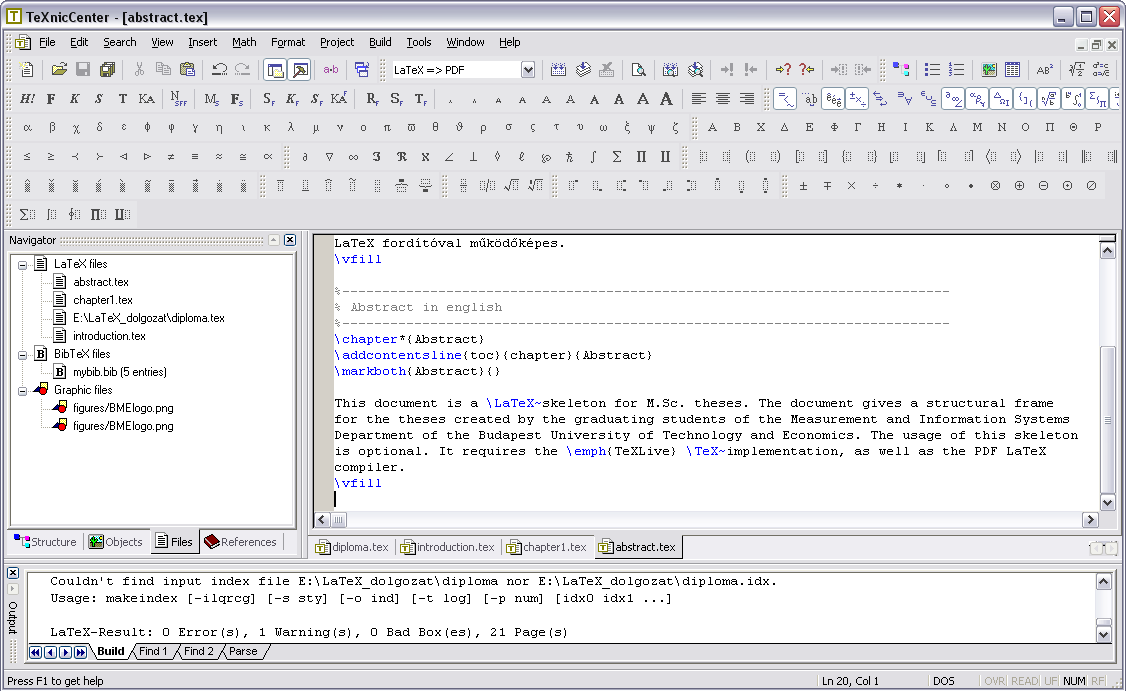
\includegraphics[width=150mm, keepaspectratio]{figures/TeXnicCenter.png}
\caption{A TeXnicCenter Windows alapú \LaTeX-szerkesztõ.} 
\end{figure}

%----------------------------------------------------------------------------
\clearpage\section{Válasz az ,,Élet, a világmindenség, meg minden'' kérdésére}
%----------------------------------------------------------------------------
A Pitagorasz-tételbõl levezetve
\begin{align}
c^2=a^2+b^2=42.
\end{align}
A Faraday-indukciós törvénybõl levezetve
\begin{align}
\rot E=-\frac{dB}{dt}\hspace{1cm}\longrightarrow \hspace{1cm}
U_i=\oint\limits_\mathbf{L}{\mathbf{E}\mathbf{dl}}=-\frac{d}{dt}\int\limits_A{\mathbf{B}\mathbf{da}}=42.
\end{align}







\label{page:last}
\end{document}
